\chapter{Introduction to Computational Science}

\section{Learning Objectives}

Upon completion of this chapter, students should be able to:

\begin{enumerate}
  \item Define computational science and explain its interdisciplinary nature
  \item Identify the three pillars of computational science and understand their interconnected relationship
  \item Understand the role of computational thinking in problem-solving across various domains
  \item Recognize applications of computational science across diverse fields including physics, biology, economics, and engineering
  \item Distinguish between different types of computational models and their appropriate applications
  \item Explain the computational science workflow and methodology for systematic problem-solving
  \item Appreciate the tripartite approach that distinguishes computational science from traditional scientific methods
  \item Understand how computational science bridges theoretical and experimental approaches to scientific inquiry
\end{enumerate}

\begin{figure}[ht]
  \centering
  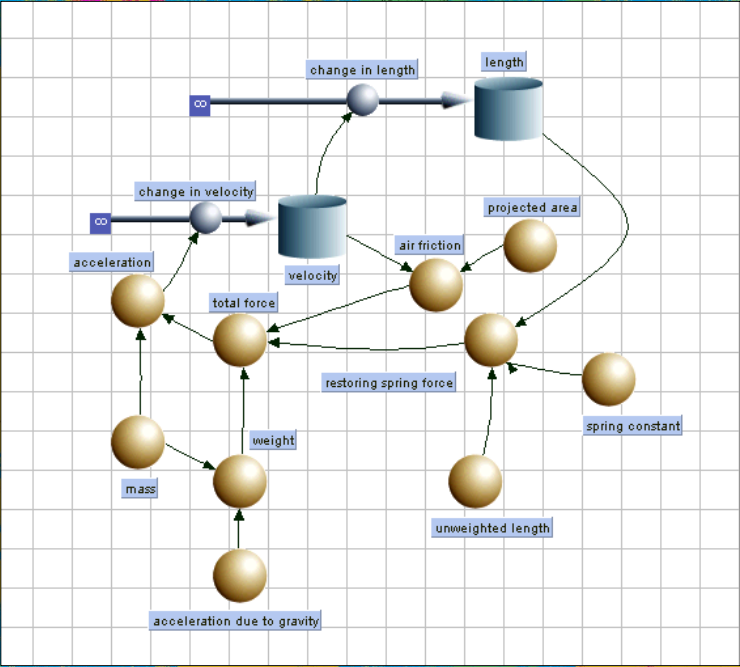
\includegraphics[width=0.8\textwidth]{images/chapter1_title_simulation.png}
  \caption{Mass-Spring Dynamics Simulation}
  \label{fig:chapter1_title}
\end{figure}

Figure~\ref{fig:chapter1_title} shows the computational modeling of a physical system with interconnected masses, springs, and forces including gravity, air friction, and restoring forces.

\section{Mass-Spring Dynamics Simulation}

\subsection{What is Mass-Spring Dynamics?}

\begin{conceptcard}{Mass-Spring Dynamics Definition}
\textbf{Mass-Spring Dynamics} is a fundamental physical and computational model that describes the behavior of systems consisting of point masses connected by elastic springs. This model serves as a cornerstone in physics, engineering, and computational science for understanding oscillatory motion, mechanical vibrations, and complex multi-body systems.
\end{conceptcard}

Mass-Spring Dynamics represents one of the most important and widely applicable models in computational physics. At its core, it describes how objects with mass respond to forces, particularly the restoring forces exerted by springs and the influence of external forces such as gravity and friction.

\subsubsection{Fundamental Components of Mass-Spring Systems}

A mass-spring system consists of several key elements that work together to create complex dynamic behaviors:

\begin{enumerate}
    \item \textbf{Point Masses}: These represent objects with mass but negligible size, characterized by:
    \begin{itemize}
        \item Mass value (m) that determines inertial properties
        \item Position coordinates (x, y, z) in space
        \item Velocity components that describe motion
        \item Acceleration determined by applied forces
    \end{itemize}
    
    \item \textbf{Springs}: Elastic connectors that exert forces proportional to displacement:
    \begin{itemize}
        \item Spring constant (k) indicating stiffness
        \item Natural (rest) length when no force is applied
        \item Current length based on connected mass positions
        \item Restoring force that opposes deformation
    \end{itemize}
    
    \item \textbf{External Forces}: Environmental influences affecting the system:
    \begin{itemize}
        \item Gravitational acceleration pulling masses downward
        \item Air resistance opposing motion
        \item Applied forces from user interaction or external sources
        \item Constraint forces maintaining system integrity
    \end{itemize}
    
    \item \textbf{Damping Elements}: Energy dissipation mechanisms:
    \begin{itemize}
        \item Viscous damping proportional to velocity
        \item Friction forces opposing motion
        \item Energy loss that causes oscillations to decay over time
    \end{itemize}
\end{enumerate}

\subsubsection{Physical Principles Governing Mass-Spring Dynamics}

The behavior of mass-spring systems is governed by fundamental laws of physics that can be expressed mathematically:

\begin{enumerate}
    \item \textbf{Newton's Second Law of Motion}:
    \begin{equation}
        \vec{F}_{net} = m\vec{a}
    \end{equation}
    where the net force on a mass determines its acceleration.
    
    \item \textbf{Hooke's Law for Elastic Springs}:
    \begin{equation}
        \vec{F}_{spring} = -k(\vec{L} - \vec{L_0})
    \end{equation}
    where:
    \begin{itemize}
        \item k is the spring constant (stiffness)
        \item $\vec{L}$ is the current spring vector
        \item $\vec{L_0}$ is the natural length vector
        \item The negative sign indicates the force opposes displacement
    \end{itemize}
    
    \item \textbf{Damping Forces}:
    \begin{equation}
        \vec{F}_{damping} = -c\vec{v}
    \end{equation}
    where c is the damping coefficient and $\vec{v}$ is the velocity vector.
    
    \item \textbf{Energy Conservation Principles}:
    \begin{itemize}
        \item Kinetic energy: $KE = \frac{1}{2}mv^2$
        \item Potential energy: $PE = \frac{1}{2}kx^2$ (for springs)
        \item Total mechanical energy in ideal systems without damping
    \end{itemize}
\end{enumerate}

\subsubsection{Applications of Mass-Spring Dynamics}

Mass-spring dynamics finds applications across numerous fields, making it a versatile and important computational model:

\begin{itemize}
    \item \textbf{Mechanical Engineering}:
    \begin{itemize}
        \item Vehicle suspension system design and analysis
        \item Vibration isolation in machinery and equipment
        \item Structural dynamics of buildings and bridges
        \item Shock absorber optimization
    \end{itemize}
    
    \item \textbf{Computer Graphics and Animation}:
    \begin{itemize}
        \item Realistic cloth and fabric simulation
        \item Hair and fur dynamics in character animation
        \item Soft body deformation in games and movies
        \item Particle system effects and simulations
    \end{itemize}
    
    \item \textbf{Robotics and Control Systems}:
    \begin{itemize}
        \item Robot arm dynamics and control
        \item Walking and running gait analysis
        \item Flexible manipulator modeling
        \item Bio-inspired locomotion systems
    \end{itemize}
    
    \item \textbf{Physics Education and Research}:
    \begin{itemize}
        \item Demonstrating oscillatory motion principles
        \item Understanding resonance and frequency response
        \item Exploring chaos and nonlinear dynamics
        \item Modeling molecular and atomic interactions
    \end{itemize}
    
    \item \textbf{Biomechanics and Medical Applications}:
    \begin{itemize}
        \item Modeling human joint and muscle dynamics
        \item Prosthetic device design and optimization
        \item Heart valve mechanics simulation
        \item Tissue elasticity and deformation studies
    \end{itemize}
\end{itemize}

\subsubsection{Computational Challenges in Mass-Spring Dynamics}

Simulating mass-spring systems computationally presents several important challenges that illustrate key concepts in computational science:

\begin{enumerate}
    \item \textbf{Numerical Integration}:
    \begin{itemize}
        \item Converting continuous differential equations to discrete time steps
        \item Choosing appropriate integration methods (Euler, Runge-Kutta, Verlet)
        \item Balancing accuracy with computational efficiency
        \item Maintaining stability over long simulation periods
    \end{itemize}
    
    \item \textbf{Time Step Selection}:
    \begin{itemize}
        \item Ensuring numerical stability with appropriate step sizes
        \item Handling stiff systems with very different time scales
        \item Adaptive time stepping for optimal performance
        \item Trade-offs between accuracy and real-time performance
    \end{itemize}
    
    \item \textbf{Force Calculation Optimization}:
    \begin{itemize}
        \item Efficient algorithms for computing spring forces
        \item Spatial data structures for neighbor finding
        \item Parallel processing for large-scale systems
        \item Memory management for complex connectivity patterns
    \end{itemize}
    
    \item \textbf{Energy Conservation and Stability}:
    \begin{itemize}
        \item Monitoring total system energy over time
        \item Preventing numerical energy gain or loss
        \item Implementing energy-conserving integration schemes
        \item Handling energy dissipation through damping
    \end{itemize}
\end{enumerate}

\subsubsection{Why Mass-Spring Dynamics is Important for Computational Science}

Mass-spring dynamics serves as an excellent introduction to computational science for several reasons:

\begin{highlightbox}{Educational Value of Mass-Spring Systems}
\begin{itemize}
    \item \textbf{Intuitive Physics}: Everyone can understand springs and masses from everyday experience
    \item \textbf{Mathematical Tractability}: Simple enough to analyze mathematically but complex enough to be interesting
    \item \textbf{Visual Appeal}: Results can be easily visualized and animated
    \item \textbf{Scalable Complexity}: Can start simple and add complexity incrementally
    \item \textbf{Interdisciplinary Connections}: Links physics, mathematics, and computer science naturally
    \item \textbf{Practical Relevance}: Has real-world applications students can relate to
\end{itemize}
\end{highlightbox}

The mass-spring model exemplifies how computational science transforms abstract mathematical concepts into concrete, observable simulations that enhance understanding and enable prediction of complex behaviors that would be difficult to analyze purely theoretically or experimentally.

\subsection{Understanding Mass-Spring Dynamics: A Computational Science Example}

Figure \ref{fig:chapter1_title} provides an excellent illustration of how computational science transforms real-world physical phenomena into mathematical models that can be simulated and analyzed computationally. This mass-spring dynamics simulation demonstrates the core principles of computational science through a tangible, observable system.

\subsubsection{The Physical System}

The mass-spring system represents one of the fundamental models in physics and engineering, consisting of:

\begin{itemize}
  \item \textbf{Point Masses}: Represented by the spherical objects in the simulation, each having specific mass properties that determine their inertial response to applied forces
  \item \textbf{Springs}: Connecting elements that exert restoring forces proportional to their displacement from equilibrium, following Hooke's Law ($F = -kx$)
  \item \textbf{Damping Elements}: Air friction and other dissipative forces that remove energy from the system over time
  \item \textbf{External Forces}: Gravitational acceleration and other environmental influences acting on the masses
\end{itemize}

\subsubsection{Mathematical Modeling Components}

The simulation incorporates several key physical principles translated into mathematical form:

\begin{enumerate}
  \item \textbf{Newton's Second Law}: $F = ma$ governs the motion of each mass, where the net force determines acceleration
      
  \item \textbf{Hooke's Law for Springs}: $F_{spring} = -k(L - L_0)$ where:
  \begin{itemize}
    \item $k$ is the spring constant (stiffness)
    \item $L$ is the current length
    \item $L_0$ is the natural (rest) length
  \end{itemize}
      
  \item \textbf{Damping Forces}: $F_{damping} = -c \cdot v$ where $c$ is the damping coefficient and $v$ is velocity
      
  \item \textbf{Gravitational Force}: $F_{gravity} = mg$ acting downward on each mass
\end{enumerate}

\subsubsection{Computational Implementation}

The simulation demonstrates how mathematical models are transformed into computational algorithms:

\begin{itemize}
  \item \textbf{Numerical Integration}: Converting continuous differential equations into discrete time steps using methods like Euler's method or Runge-Kutta algorithms
  \item \textbf{Force Calculation}: Computing the net force on each mass by summing contributions from all springs, damping, and external forces
  \item \textbf{Position Updates}: Using numerical integration to update positions and velocities at each time step
  \item \textbf{Constraint Handling}: Managing boundary conditions and connection constraints between masses
  \item \textbf{Real-time Visualization}: Rendering the dynamic system state for observation and analysis
\end{itemize}

\subsubsection{Interdisciplinary Nature Demonstrated}

This example perfectly illustrates the tripartite nature of computational science:

\begin{itemize}
  \item \textbf{Domain Science (Physics)}: Understanding of mechanics, forces, energy conservation, and material properties
  \item \textbf{Mathematical Modeling}: Translation of physical laws into differential equations and mathematical relationships
  \item \textbf{Computer Science}: Algorithm design, numerical methods, data structures for efficient computation, and visualization techniques
\end{itemize}

\subsubsection{Educational and Research Applications}

Mass-spring simulations serve multiple purposes in computational science education and research:

\begin{itemize}
  \item \textbf{Concept Demonstration}: Visualizing abstract physical principles like oscillation, resonance, and energy transfer
  \item \textbf{Parameter Studies}: Exploring how changes in mass, spring constants, or damping affect system behavior
  \item \textbf{Validation Studies}: Comparing computational results with analytical solutions for simple cases
  \item \textbf{Method Development}: Testing new numerical integration schemes and computational algorithms
  \item \textbf{Engineering Applications}: Modeling vibrations in structures, vehicle suspension systems, and mechanical assemblies
\end{itemize}

\subsubsection{Computational Challenges and Considerations}

The simulation also highlights important computational science considerations:

\begin{itemize}
  \item \textbf{Numerical Stability}: Ensuring the simulation remains stable over long time periods
  \item \textbf{Time Step Selection}: Balancing computational efficiency with accuracy
  \item \textbf{Energy Conservation}: Monitoring whether the numerical scheme preserves physical conservation laws
  \item \textbf{Performance Optimization}: Efficient algorithms for force calculations and collision detection
  \item \textbf{Scalability}: Handling systems with large numbers of interconnected masses and springs
\end{itemize}

This mass-spring dynamics example thus serves as a microcosm of computational science, demonstrating how real-world phenomena are systematically transformed into computational models that provide insights, predictions, and understanding that would be difficult or impossible to achieve through purely theoretical or experimental approaches alone.

\section{What is Computational Science?}

\begin{conceptcard}{Definition of Computational Science}
\textbf{Computational Science} is an interdisciplinary field that uses mathematical models, quantitative analysis techniques, and computer simulations to solve complex problems in science, engineering, business, and other domains. It combines the power of computing with mathematical modeling and scientific theory to understand and predict real-world phenomena through the creation and analysis of computational models.
\end{conceptcard}

Computational science represents a paradigm shift in how we approach scientific inquiry and problem-solving. Unlike traditional experimental and theoretical approaches, computational science offers a ``third pillar'' of scientific discovery that complements laboratory experiments and mathematical theory. This field has emerged as a critical component of modern research due to the increasing complexity of problems that cannot be adequately addressed through experimentation or theory alone.

The essence of computational science lies in its ability to create virtual laboratories where researchers can conduct experiments that would be impossible, too dangerous, too expensive, or too time-consuming to perform in reality. For instance, we can simulate the formation of galaxies over billions of years, model the spread of infectious diseases across populations, or test the structural integrity of buildings under various earthquake conditions.

\subsection{The Evolution of Scientific Methodology}

Historically, science has progressed through two primary approaches:

\begin{enumerate}
  \item \textbf{Empirical/Experimental Science}: Direct observation and experimentation to understand natural phenomena
  \item \textbf{Theoretical Science}: Mathematical formulation of natural laws and principles
\end{enumerate}

The 20th and 21st centuries have witnessed the emergence of a third approach—computational science—which bridges the gap between theory and experiment by enabling the exploration of complex systems through simulation and modeling.

\begin{figure}[h]
 \centering
 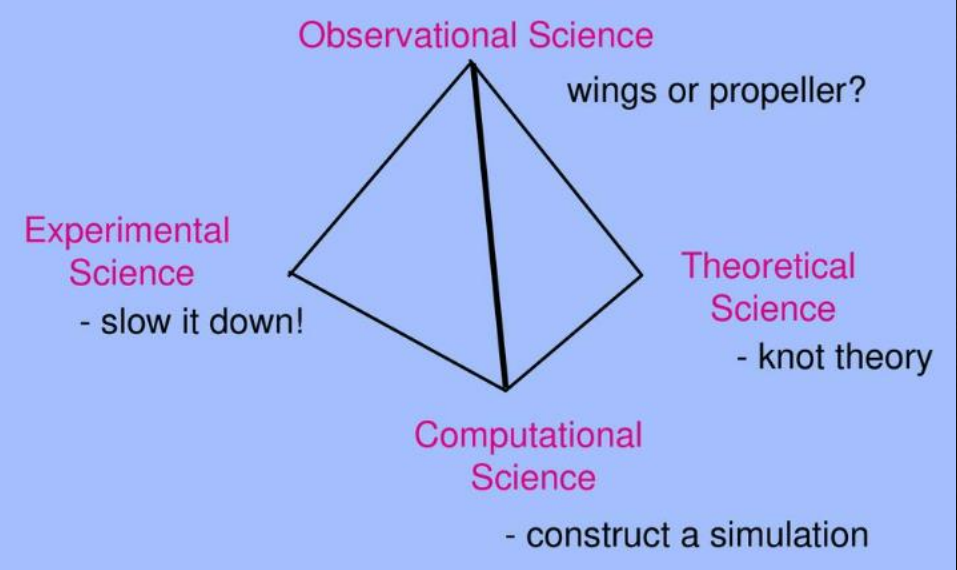
\includegraphics[width=0.8\textwidth]{images/science_four_pillars.png}
 \caption{Four Pillars of Computational Science}
 \label{fig:science_pillars}
\end{figure}

Figure~\ref{fig:science_pillars} illustrates the four complementary approaches to scientific discovery: Observational Science (observing natural phenomena), Experimental Science (controlled experiments), Theoretical Science (mathematical formulation), and Computational Science (simulation and modeling).

\subsection{The Four Pillars of Scientific Discovery}

The pyramid-shaped diagram in Figure~\ref{fig:science_pillars} represents the evolution of scientific methodology from its traditional foundations to the modern interdisciplinary approach that includes computational science. Each vertex of this pyramid represents a distinct but interconnected approach to understanding how nature behaves.

\subsubsection{Observational Science: "Wings or Propeller?"}

\begin{conceptcard}{Observational Science}
\textbf{Observational Science} involves the systematic observation and recording of natural phenomena without direct manipulation or intervention. It focuses on describing what happens in nature through careful observation and pattern recognition.
\end{conceptcard}

Observational science represents the most fundamental approach to scientific inquiry, dating back to ancient civilizations. The phrase "wings or propeller?" in the diagram captures the essence of observational science—asking questions about what we see and trying to understand the mechanisms behind observable phenomena.

\textbf{Characteristics of Observational Science:}
\begin{itemize}
    \item \textbf{Passive Data Collection}: Scientists observe and record phenomena as they naturally occur
    \item \textbf{Pattern Recognition}: Identifying trends, cycles, and relationships in observed data
    \item \textbf{Descriptive Analysis}: Cataloging and classifying natural phenomena
    \item \textbf{Hypothesis Generation}: Developing initial theories based on observations
    \item \textbf{Long-term Studies}: Monitoring changes over extended periods
\end{itemize}

\textbf{Examples of Observational Science:}
\begin{itemize}
    \item Astronomy: Observing celestial objects and cosmic phenomena
    \item Ecology: Studying animal behavior and ecosystem dynamics
    \item Meteorology: Weather pattern observation and climate monitoring
    \item Epidemiology: Disease outbreak tracking and health pattern analysis
    \item Geology: Rock formation studies and geological process observation
\end{itemize}

\subsubsection{Experimental Science: "Slow it Down!"}

\begin{conceptcard}{Experimental Science}
\textbf{Experimental Science} involves controlled manipulation of variables to test hypotheses and establish cause-and-effect relationships. The motto "slow it down!" reflects the methodical, controlled approach of experimental investigation.
\end{conceptcard}

Experimental science revolutionized our understanding of the natural world by introducing controlled conditions and systematic variable manipulation. This approach allows scientists to isolate specific factors and determine their individual effects on observed phenomena.

\textbf{Key Principles of Experimental Science:}
\begin{itemize}
    \item \textbf{Controlled Variables}: Maintaining constant conditions except for the factor being tested
    \item \textbf{Reproducibility}: Ensuring experiments can be repeated with consistent results
    \item \textbf{Isolation of Effects}: Studying one variable at a time to understand its specific impact
    \item \textbf{Statistical Analysis}: Using quantitative methods to validate results
    \item \textbf{Peer Review}: Subjecting findings to scrutiny by the scientific community
\end{itemize}

\textbf{Experimental Method Components:}
\begin{enumerate}
    \item \textbf{Hypothesis Formation}: Developing testable predictions based on observations
    \item \textbf{Experimental Design}: Planning controlled procedures to test hypotheses
    \item \textbf{Data Collection}: Gathering quantitative and qualitative measurements
    \item \textbf{Analysis and Interpretation}: Drawing conclusions from experimental results
    \item \textbf{Validation and Replication}: Confirming findings through repeated experiments
\end{enumerate}

\subsubsection{Theoretical Science: "Knot Theory"}

\begin{conceptcard}{Theoretical Science}
\textbf{Theoretical Science} involves developing mathematical models, frameworks, and abstract theories to explain natural phenomena. The reference to "knot theory" exemplifies how complex mathematical concepts can describe and predict natural behaviors.
\end{conceptcard}

Theoretical science provides the mathematical foundation for understanding natural laws and principles. It transforms observations and experimental findings into elegant mathematical formulations that can predict behavior and reveal underlying patterns.

\textbf{Components of Theoretical Science:}
\begin{itemize}
    \item \textbf{Mathematical Modeling}: Creating mathematical representations of physical phenomena
    \item \textbf{Abstract Reasoning}: Developing conceptual frameworks beyond direct observation
    \item \textbf{Predictive Capability}: Using theories to forecast future states or behaviors
    \item \textbf{Unification}: Connecting seemingly disparate phenomena under common principles
    \item \textbf{Elegance and Simplicity}: Seeking the most fundamental explanations
\end{itemize}

\textbf{Examples of Theoretical Contributions:}
\begin{itemize}
    \item Einstein's Theory of Relativity: Unified space, time, and gravity
    \item Quantum Mechanics: Mathematical description of subatomic behavior
    \item Thermodynamics: Statistical mechanics of energy and entropy
    \item Information Theory: Mathematical foundation of communication and computation
    \item Knot Theory: Mathematical study of knots with applications in DNA structure and physics
\end{itemize}

\subsubsection{Computational Science: "Construct a Simulation"}

\begin{conceptcard}{Computational Science}
\textbf{Computational Science} represents the newest pillar of scientific discovery, using computer simulations and numerical analysis to explore complex systems that are difficult to study through observation, experimentation, or pure theory alone.
\end{conceptcard}

The directive to "construct a simulation" captures the essence of computational science—creating virtual representations of real-world phenomena that can be manipulated, tested, and analyzed in ways that would be impossible with traditional approaches.

\textbf{Unique Capabilities of Computational Science:}
\begin{itemize}
    \item \textbf{Virtual Experimentation}: Conducting experiments that are impossible in reality
    \item \textbf{Scale Bridging}: Connecting phenomena across vastly different spatial and temporal scales
    \item \textbf{Parameter Exploration}: Testing thousands of scenarios rapidly and systematically
    \item \textbf{Visualization}: Making invisible phenomena visible and understandable
    \item \textbf{Prediction}: Forecasting future states based on current conditions and known laws
\end{itemize}

\textbf{Computational Approaches:}
\begin{enumerate}
    \item \textbf{Numerical Simulation}: Solving mathematical models computationally
    \item \textbf{Data Analysis}: Processing large datasets to extract patterns and insights
    \item \textbf{Machine Learning}: Using algorithms to identify patterns and make predictions
    \item \textbf{Visualization}: Creating graphical representations of complex data and phenomena
    \item \textbf{Optimization}: Finding optimal solutions to complex problems
\end{enumerate}

\subsection{The Synergistic Diamond: Integrating Four Approaches}

The diamond configuration in Figure~\ref{fig:science_pillars} is not merely a geometric arrangement—it represents the interconnected and complementary nature of these four scientific approaches. Each pillar contributes unique strengths while addressing the limitations of the others:

\begin{itemize}
    \item \textbf{Observational-Experimental Synergy}: Observations guide experimental design, while experiments validate or refute observational hypotheses
    \item \textbf{Theoretical-Computational Integration}: Theories provide the mathematical foundation for simulations, while computational results test theoretical predictions
    \item \textbf{Cross-Pillar Validation}: Findings from one approach can be validated through methods from other pillars
    \item \textbf{Complementary Perspectives}: Each approach reveals different aspects of the same natural phenomena
\end{itemize}

\begin{highlightbox}{The Power of Integration}
Modern scientific breakthroughs increasingly emerge from the integration of all four approaches:
\begin{itemize}
    \item \textbf{Climate Science}: Combines observational data, laboratory experiments, theoretical models, and computational simulations
    \item \textbf{Drug Discovery}: Integrates biological observations, controlled experiments, theoretical chemistry, and computational molecular modeling
    \item \textbf{Astrophysics}: Merges telescopic observations, laboratory plasma experiments, theoretical physics, and numerical cosmological simulations
    \item \textbf{Materials Science}: Unifies structural observations, experimental testing, theoretical solid-state physics, and computational materials design
\end{itemize}
\end{highlightbox}

\subsection{The Tripartite Nature of Computational Science}

One of the most significant aspects of computational science is its tripartite structure, which integrates three essential components into a cohesive methodology. This approach distinguishes computational science from other computational fields and establishes it as a unique scientific discipline.

\begin{conceptcard}{The Tripartite Foundation}
The \textbf{Tripartite Approach} to computational science recognizes that effective computational research requires the seamless integration of three fundamental pillars: \textbf{Architecture} (Computing Environment), \textbf{Algorithm} (Mathematical Model), and \textbf{Application} (Science). These three components work synergistically to create computational models that bridge theory and practice.
\end{conceptcard}

\subsection{Understanding the Tripartite Triangle}

\begin{figure}[h]
 \centering
 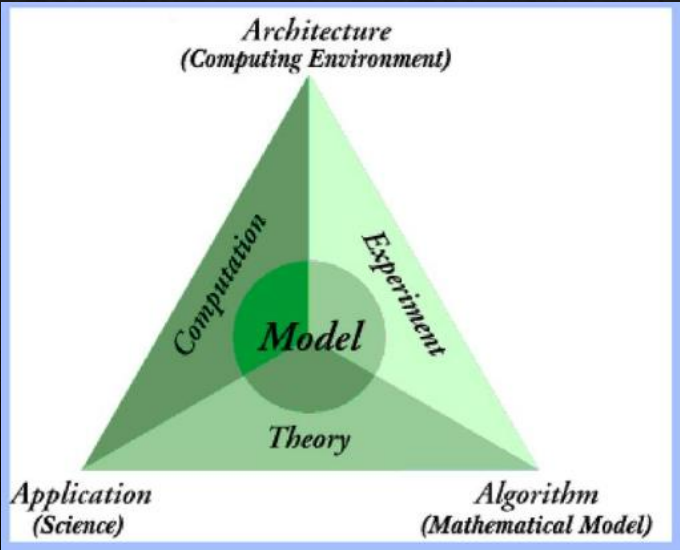
\includegraphics[width=0.7\textwidth]{images/tripartite_triangle.png}
 \caption{Tripartite Approach to Computational Science}
 \label{fig:tripartite_approach}
\end{figure}

Figure~\ref{fig:tripartite_approach} illustrates the tripartite approach as a triangle with three vertices representing the fundamental components of computational science. This geometric representation is not merely symbolic—it reflects the inherent interdependence and balance required among these components for successful computational science endeavors.

The triangle's structure emphasizes several key principles:

\begin{itemize}
    \item \textbf{Equality of Importance}: Each vertex represents an equally crucial component; weakness in any one area compromises the entire endeavor
    \item \textbf{Interconnectedness}: The edges of the triangle represent the critical interfaces between components
    \item \textbf{Central Integration}: The model at the center emerges from the synthesis of all three components
    \item \textbf{Dynamic Balance}: Success requires maintaining balance among all three aspects throughout the research process
\end{itemize}

\subsubsection{Vertex 1: Architecture (Computing Environment)}

\begin{conceptcard}{Architecture - The Computing Foundation}
\textbf{Architecture} encompasses the entire computational infrastructure that enables scientific computing, from hardware platforms and software frameworks to programming paradigms and system design principles. It represents the "how" of computational implementation.
\end{conceptcard}

The Architecture vertex addresses the fundamental computational infrastructure questions that determine what is computationally feasible and how efficiently it can be accomplished.

\textbf{Hardware Architecture Components:}
\begin{itemize}
    \item \textbf{Processing Units}: CPUs, GPUs, specialized processors (FPGAs, TPUs)
    \item \textbf{Memory Hierarchy}: RAM, cache systems, storage architectures
    \item \textbf{Network Infrastructure}: High-speed interconnects, distributed computing networks
    \item \textbf{Parallel Computing Platforms}: Shared memory, distributed memory, hybrid systems
    \item \textbf{Accelerator Technologies}: Graphics cards, quantum processors, neuromorphic chips
\end{itemize}

\textbf{Software Architecture Elements:}
\begin{itemize}
    \item \textbf{Programming Languages}: Python, C/C++, Fortran, Julia, R, MATLAB
    \item \textbf{Development Frameworks}: Scientific computing libraries, parallel programming models
    \item \textbf{Runtime Systems}: Operating systems, job schedulers, resource managers
    \item \textbf{Development Tools}: Compilers, debuggers, profilers, version control systems
    \item \textbf{Middleware}: Database systems, visualization tools, workflow management
\end{itemize}

\textbf{Computational Paradigms:}
\begin{itemize}
    \item \textbf{High-Performance Computing}: Supercomputing, cluster computing
    \item \textbf{Cloud Computing}: On-demand resources, scalable infrastructure
    \item \textbf{Edge Computing}: Distributed processing, real-time computation
    \item \textbf{Grid Computing}: Resource sharing across institutions
    \item \textbf{Quantum Computing}: Quantum algorithms, quantum simulators
\end{itemize}

\textbf{Architecture Considerations:}
\begin{itemize}
    \item \textbf{Performance Optimization}: Maximizing computational throughput and minimizing execution time
    \item \textbf{Scalability}: Handling increasing problem sizes and computational demands
    \item \textbf{Resource Efficiency}: Optimal utilization of computational resources
    \item \textbf{Reliability}: Ensuring system stability and fault tolerance
    \item \textbf{Accessibility}: Making computational resources available to researchers
\end{itemize}

\subsubsection{Vertex 2: Algorithm (Mathematical Model)}

\begin{conceptcard}{Algorithm - The Mathematical Foundation}
\textbf{Algorithm} represents the mathematical and computational methods that transform real-world problems into solvable computational forms. It encompasses both the mathematical modeling of phenomena and the algorithmic approaches for solving the resulting equations.
\end{conceptcard}

The Algorithm vertex bridges the gap between abstract mathematical descriptions of natural phenomena and concrete computational procedures that can be executed on computing systems.

\textbf{Mathematical Modeling Components:}
\begin{itemize}
    \item \textbf{Differential Equations}: Ordinary and partial differential equations describing dynamic systems
    \item \textbf{Statistical Models}: Probabilistic descriptions of uncertain phenomena
    \item \textbf{Optimization Models}: Mathematical formulations of decision problems
    \item \textbf{Discrete Models}: Graph theory, combinatorial optimization, cellular automata
    \item \textbf{Stochastic Models}: Random processes, Monte Carlo methods, uncertainty quantification
\end{itemize}

\textbf{Numerical Methods:}
\begin{itemize}
    \item \textbf{Numerical Integration}: Euler methods, Runge-Kutta schemes, multistep methods
    \item \textbf{Linear Algebra}: Matrix operations, eigenvalue problems, iterative solvers
    \item \textbf{Finite Element Methods}: Spatial discretization for partial differential equations
    \item \textbf{Finite Difference Methods}: Grid-based approximations of derivatives
    \item \textbf{Spectral Methods}: Fourier and polynomial-based solution techniques
\end{itemize}

\textbf{Algorithmic Design Principles:}
\begin{itemize}
    \item \textbf{Accuracy}: Ensuring numerical solutions accurately represent the mathematical model
    \item \textbf{Stability}: Maintaining solution reliability over long computational runs
    \item \textbf{Efficiency}: Minimizing computational complexity and resource requirements
    \item \textbf{Robustness}: Handling edge cases and numerical difficulties gracefully
    \item \textbf{Parallelizability}: Designing algorithms suitable for parallel execution
\end{itemize}

\textbf{Error Analysis and Control:}
\begin{itemize}
    \item \textbf{Discretization Error}: Errors from approximating continuous problems
    \item \textbf{Round-off Error}: Accumulation of floating-point arithmetic errors
    \item \textbf{Convergence Analysis}: Theoretical guarantees for algorithm behavior
    \item \textbf{Adaptive Methods}: Dynamic adjustment of computational parameters
    \item \textbf{Uncertainty Quantification}: Propagation of input uncertainties through calculations
\end{itemize}

\subsubsection{Vertex 3: Application (Science)}

\begin{conceptcard}{Application - The Scientific Foundation}
\textbf{Application} represents the domain-specific scientific knowledge, understanding, and expertise that drives computational science research. It encompasses the scientific questions, physical understanding, and validation criteria that give meaning and context to computational investigations.
\end{conceptcard}

The Application vertex ensures that computational science serves real scientific purposes and produces meaningful, interpretable, and actionable results within specific scientific domains.

\textbf{Domain-Specific Knowledge:}
\begin{itemize}
    \item \textbf{Physical Sciences}: Physics, chemistry, astronomy, materials science
    \item \textbf{Life Sciences}: Biology, medicine, ecology, bioinformatics
    \item \textbf{Earth Sciences}: Climatology, geology, oceanography, atmospheric science
    \item \textbf{Engineering}: Mechanical, electrical, aerospace, civil engineering
    \item \textbf{Social Sciences}: Economics, sociology, political science, psychology
\end{itemize}

\textbf{Scientific Methodology:}
\begin{itemize}
    \item \textbf{Problem Formulation}: Translating scientific questions into computational problems
    \item \textbf{Hypothesis Development}: Creating testable predictions from computational models
    \item \textbf{Experimental Design}: Planning computational experiments and parameter studies
    \item \textbf{Data Analysis}: Interpreting computational results in scientific context
    \item \textbf{Validation Studies}: Comparing computational predictions with empirical data
\end{itemize}

\textbf{Scientific Understanding Requirements:}
\begin{itemize}
    \item \textbf{Fundamental Principles}: Deep understanding of governing physical laws and relationships
    \item \textbf{Phenomenological Knowledge}: Awareness of relevant phenomena and their characteristics
    \item \textbf{Scale Considerations}: Understanding of relevant temporal and spatial scales
    \item \textbf{Limiting Cases}: Knowledge of simplified scenarios and analytical solutions
    \item \textbf{Physical Intuition}: Ability to assess whether computational results are reasonable
\end{itemize}

\textbf{Validation and Verification:}
\begin{itemize}
    \item \textbf{Model Validation}: Ensuring models accurately represent real-world phenomena
    \item \textbf{Experimental Comparison}: Benchmarking against laboratory and field measurements
    \item \textbf{Cross-Validation}: Comparing different computational approaches
    \item \textbf{Sensitivity Analysis}: Understanding model response to parameter variations
    \item \textbf{Uncertainty Assessment}: Quantifying confidence in computational predictions
\end{itemize}

\subsubsection{The Central Model: Synthesis and Integration}

\begin{conceptcard}{The Computational Model}
The \textbf{Model} at the center of the tripartite triangle represents the integrated computational representation that emerges from the synthesis of Architecture, Algorithm, and Application. It is the concrete manifestation of computational science that enables scientific discovery and understanding.
\end{conceptcard}

The central model is not simply the sum of its three components—it represents a new entity that emerges from their integration and interaction. This model embodies the unique value proposition of computational science: the ability to explore, predict, and understand complex phenomena through computational means.

\textbf{Model Characteristics:}
\begin{itemize}
    \item \textbf{Computational Representation}: Digital encoding of scientific phenomena
    \item \textbf{Predictive Capability}: Ability to forecast future states or behaviors
    \item \textbf{Exploratory Power}: Capacity to investigate scenarios impossible in reality
    \item \textbf{Scalable Complexity}: Capability to handle problems across different scales
    \item \textbf{Interactive Analysis}: Real-time exploration and parameter manipulation
\end{itemize}

\textbf{Model Functions:}
\begin{itemize}
    \item \textbf{Virtual Experimentation}: Conducting experiments in computational space
    \item \textbf{Hypothesis Testing}: Evaluating scientific theories and predictions
    \item \textbf{Parameter Space Exploration}: Systematic investigation of model behaviors
    \item \textbf{Optimization}: Finding optimal designs or operating conditions
    \item \textbf{Sensitivity Analysis}: Understanding factor importance and model robustness
\end{itemize}

\subsection{The Synergistic Relationships: Triangle Edges}

The edges of the tripartite triangle represent the critical interfaces and relationships between the three fundamental components. These relationships are bidirectional and essential for successful computational science.

\subsubsection{Architecture-Algorithm Interface}

The relationship between Architecture and Algorithm involves the optimization of computational methods for specific hardware platforms and the design of algorithms that can effectively utilize available computational resources.

\textbf{Key Considerations:}
\begin{itemize}
    \item \textbf{Algorithm-Hardware Matching}: Choosing algorithms suited to available computational architectures
    \item \textbf{Performance Optimization}: Tuning algorithms for specific hardware characteristics
    \item \textbf{Parallel Algorithm Design}: Developing algorithms that can exploit parallel processing capabilities
    \item \textbf{Memory Management}: Optimizing data access patterns for hierarchical memory systems
    \item \textbf{Scalability Planning}: Ensuring algorithms can utilize larger computational resources effectively
\end{itemize}

\subsubsection{Algorithm-Application Interface}

The Algorithm-Application interface focuses on ensuring that mathematical models and computational methods accurately capture the essential physics and behavior of the scientific system under study.

\textbf{Key Considerations:}
\begin{itemize}
    \item \textbf{Physical Fidelity}: Ensuring mathematical models represent relevant physics
    \item \textbf{Approximation Assessment}: Understanding the impact of mathematical simplifications
    \item \textbf{Scale Matching}: Choosing mathematical approaches appropriate for the relevant scales
    \item \textbf{Validation Requirements}: Designing computational methods that can be validated against data
    \item \textbf{Scientific Interpretation}: Ensuring computational results can be interpreted scientifically
\end{itemize}

\subsubsection{Application-Architecture Interface}

The Application-Architecture relationship involves understanding how scientific requirements drive computational resource needs and how computational limitations constrain scientific investigations.

\textbf{Key Considerations:}
\begin{itemize}
    \item \textbf{Resource Requirements}: Estimating computational needs for scientific problems
    \item \textbf{Constraint Recognition}: Understanding how computational limitations affect scientific scope
    \item \textbf{Technology Selection}: Choosing appropriate computational tools for scientific applications
    \item \textbf{Collaboration Models}: Organizing computational resources for scientific research
    \item \textbf{Future Planning}: Anticipating computational needs for advancing scientific understanding
\end{itemize}

\subsection{Practical Implementation of the Tripartite Approach}

\begin{examplebox}{Tripartite Approach in Climate Modeling}
Consider a climate modeling project that exemplifies the tripartite approach:

\textbf{Application (Science):}
\begin{itemize}
    \item Understanding atmospheric and oceanic physics
    \item Knowledge of climate system interactions
    \item Validation against observational climate data
    \item Scientific questions about climate change impacts
\end{itemize}

\textbf{Algorithm (Mathematical Model):}
\begin{itemize}
    \item Navier-Stokes equations for fluid dynamics
    \item Radiative transfer equations for energy balance
    \item Numerical methods for partial differential equations
    \item Grid-based discretization of Earth's surface
\end{itemize}

\textbf{Architecture (Computing Environment):}
\begin{itemize}
    \item High-performance computing clusters
    \item Parallel programming with MPI
    \item Fortran and C++ implementation
    \item Distributed data storage systems
\end{itemize}

\textbf{Integrated Model:}
The resulting global climate model can simulate Earth's climate system, predict future climate scenarios, and explore the impacts of different emission pathways, demonstrating how the three components work together to enable scientific discovery.
\end{examplebox}

\subsection{Benefits of the Tripartite Approach}

The tripartite framework provides several important benefits for computational science practice:

\begin{itemize}
    \item \textbf{Systematic Planning}: Ensures all essential components are considered in project design
    \item \textbf{Balanced Development}: Prevents overemphasis on any single aspect at the expense of others
    \item \textbf{Quality Assurance}: Provides checkpoints for evaluating project progress and success
    \item \textbf{Interdisciplinary Communication}: Offers a common framework for collaboration across disciplines
    \item \textbf{Educational Structure}: Organizes computational science curriculum and training
    \item \textbf{Research Evaluation}: Provides criteria for assessing computational science contributions
\end{itemize}

\subsection{Challenges in Tripartite Integration}

While the tripartite approach provides a powerful framework, implementing it effectively presents several challenges:

\begin{itemize}
    \item \textbf{Expertise Requirements}: Few individuals possess deep knowledge in all three areas
    \item \textbf{Communication Barriers}: Different communities use different languages and approaches
    \item \textbf{Resource Allocation}: Balancing investment across the three components
    \item \textbf{Timeline Coordination}: Synchronizing development across different aspects
    \item \textbf{Quality Control}: Maintaining standards across diverse technical areas
    \item \textbf{Technology Evolution}: Keeping pace with rapid changes in all three domains
\end{itemize}

The tripartite nature of computational science thus represents both the strength and the challenge of the field—its power comes from integration across disciplines, but this integration requires careful attention to all three fundamental components and their interactions.

\subsection{The Interdisciplinary Venn Diagram Perspective}

\begin{figure}[h]
 \centering
 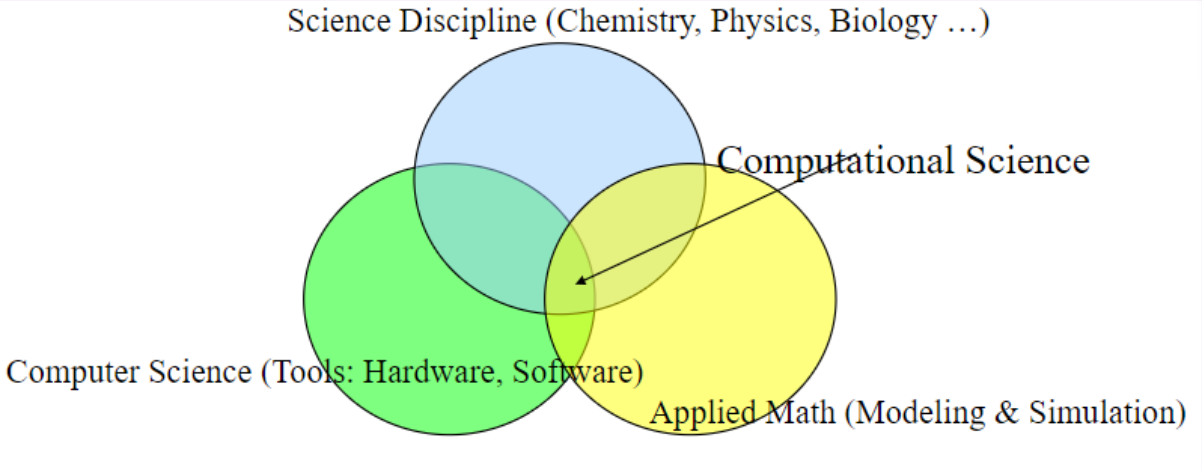
\includegraphics[width=0.8\textwidth]{images/computational_science_venn.png}
 \caption{Computational Science at the Intersection of Disciplines}
 \label{fig:computational_science_venn}
\end{figure}

Figure~\ref{fig:computational_science_venn} illustrates computational science as the intersection of three fundamental academic disciplines, forming a tripartite approach that defines the field's unique character and capabilities.

\subsubsection{The Three Foundational Disciplines}

\textbf{Science Disciplines} form the blue circle in our diagram, encompassing fields like chemistry, physics, biology, economics, and other domain sciences. These disciplines provide the fundamental questions that drive computational research and the real-world knowledge needed to validate computational results. For example, when studying climate change, atmospheric physicists provide understanding of weather patterns, while chemists contribute knowledge about greenhouse gas interactions in the atmosphere.

\textbf{Computer Science} represents the green circle, contributing the tools and methodologies for computation. This includes hardware design, software development, algorithms, and data structures that make complex calculations possible. Consider how computer scientists developed parallel processing algorithms that allow climate models to run efficiently on supercomputers, processing millions of calculations simultaneously.

\textbf{Applied Mathematics} forms the yellow circle, providing the mathematical framework that transforms real-world phenomena into solvable equations. This discipline offers modeling techniques, numerical analysis, and optimization methods that bridge abstract mathematics with practical problem-solving. For instance, mathematicians develop differential equations that describe how heat flows through the atmosphere, which can then be solved computationally.

\subsubsection{The Intersection: Where Innovation Happens}

The magic of computational science occurs at the center where all three circles overlap. This intersection creates a new discipline that is greater than the sum of its parts. A computational scientist studying drug discovery, for example, must understand the biological mechanisms of disease (science), implement machine learning algorithms to analyze molecular data (computer science), and develop statistical models to predict drug effectiveness (applied mathematics).

This interdisciplinary approach enables computational scientists to tackle problems that no single field could address alone. Weather prediction requires atmospheric science knowledge, sophisticated algorithms to process satellite data, and complex mathematical models—all working together to forecast tomorrow's conditions. The strength of computational science lies not in deep specialization within one field, but in the ability to synthesize knowledge across disciplines to solve complex, real-world problems.

\subsection{Real-World Applications Across Disciplines}

\begin{figure}[h]
 \centering
 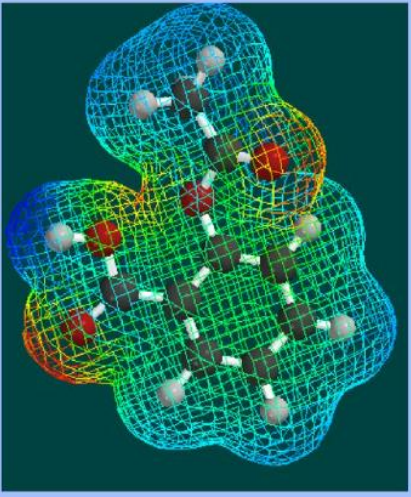
\includegraphics[width=0.6\textwidth]{images/molecular_structure.png}
 \caption{Computational Modeling of Molecular Structures}
 \label{fig:molecular_structure}
\end{figure}

The true power of computational science becomes evident when we examine its diverse applications across multiple scientific domains. Figure~\ref{fig:molecular_structure} illustrates one such application—the computational visualization of molecular structures that enables scientists to understand complex chemical interactions at the atomic level.

\subsubsection{Chemistry: Electronic Structure Determinations}

In computational chemistry, scientists use quantum mechanical calculations to determine how electrons are arranged around atoms and molecules. This electronic structure determination helps predict chemical reactions, design new materials, and understand molecular behavior. For example, pharmaceutical companies use computational methods to predict how drug molecules will interact with proteins in the human body, significantly reducing the time and cost of drug development compared to traditional laboratory experiments alone.

\subsubsection{Physics: Astrophysics and Galaxy Simulations}

Computational physics enables scientists to simulate cosmic phenomena that span billions of years and vast distances. Galaxy formation simulations help astronomers understand how the universe evolved from the Big Bang to its current state. These simulations combine gravitational physics, thermodynamics, and stellar evolution models to recreate the birth and death of stars, the formation of galaxies, and the large-scale structure of the universe—phenomena impossible to observe directly due to their immense time scales.

\subsubsection{Biology: Population Dynamics}

Computational biology models help scientists understand how populations of organisms change over time. These models can predict the spread of infectious diseases, track endangered species recovery, or analyze ecosystem stability. During the COVID-19 pandemic, computational epidemiological models became crucial tools for predicting infection rates and evaluating the effectiveness of public health interventions.

\subsubsection{Environmental Science: Acid Rain Deposition Models}

Environmental scientists use computational models to track how pollutants move through the atmosphere and affect ecosystems. Acid rain models simulate how sulfur and nitrogen compounds travel from industrial sources, undergo chemical transformations in the atmosphere, and eventually deposit in forests and lakes. These models help policymakers understand the regional impacts of pollution and design effective environmental regulations.

\subsubsection{Political Science and History: Analyzing Complex Social Phenomena}

Computational social science applies quantitative methods to understand historical events and political processes. For instance, researchers have used computational models to analyze the causative factors in the Bosnian War conflict, examining how ethnic tensions, economic factors, and political decisions interacted to escalate the situation. These models help historians and political scientists identify patterns and test theories about complex social phenomena.

\subsubsection{Medicine: Epidemiology and Pharmacokinetics}

Medical applications of computational science range from tracking disease outbreaks to modeling how drugs move through the human body. Epidemiological models help public health officials predict and control disease spread, while pharmacokinetic models help doctors determine optimal drug dosages by predicting how medications are absorbed, distributed, metabolized, and eliminated by the body. These computational tools have become indispensable for evidence-based medical practice.

The diversity of these applications demonstrates that computational science is not confined to traditional "hard" sciences but extends to any field where complex systems can be modeled mathematically and solved computationally. Each application requires the same tripartite integration of domain expertise, computational methods, and mathematical modeling that defines computational science as a discipline.

\subsection{Fundamental Algorithms in Computational Science}

\begin{figure}[h]
 \centering
 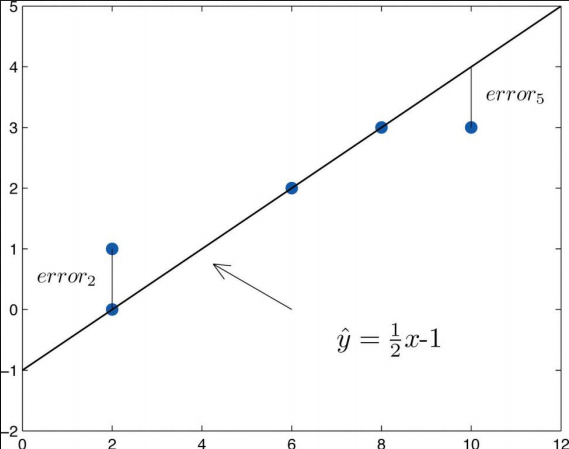
\includegraphics[width=0.6\textwidth]{images/least_squares_regression.png}
 \caption{Linear Least Squares Regression Example}
 \label{fig:least_squares_regression}
\end{figure}

At the heart of computational science lies the development and application of algorithms—systematic procedures for solving mathematical problems computationally. These algorithms serve as the bridge between theoretical mathematical models and practical computational solutions. Figure~\ref{fig:least_squares_regression} illustrates one fundamental example: the least squares regression method for fitting data to mathematical functions.

\subsubsection{The Algorithm Development Process}

Creating effective computational algorithms involves two critical steps that transform real-world problems into computable solutions:

\textbf{Mathematical Representation of the Problem}

The first step requires translating a physical phenomenon or scientific question into a mathematical framework—what we call the "mathematical model." This process involves identifying the key variables, relationships, and constraints that govern the system under study. For instance, when studying population growth, we might represent the problem using differential equations that describe how birth rates, death rates, and environmental factors influence population changes over time.

\textbf{Choosing the Appropriate Numerical Recipe}

Once we have a mathematical model, we must select or develop a numerical method—a "recipe"—that can solve the problem computationally. This choice depends on the nature of the mathematical problem, the required accuracy, available computational resources, and the specific characteristics of the data or system being studied.

\subsubsection{Essential Numerical Methods}

Computational science relies on several fundamental algorithmic approaches, each designed for specific types of mathematical problems:

\textbf{Linear Least Squares Method}

This algorithm finds the best-fitting line (or curve) through a set of data points by minimizing the sum of squared errors between the observed data and the predicted values. As shown in Figure~\ref{fig:least_squares_regression}, the method determines the line $\hat{y} = \frac{1}{2}x - 1$ that best represents the relationship between variables while accounting for measurement errors. This technique is fundamental in data analysis, experimental science, and machine learning applications.

\textbf{Newton's Method}

Newton's method provides an iterative approach for finding the roots of equations—points where a function equals zero. This algorithm is particularly powerful because it converges rapidly to solutions when given a good initial guess. Scientists use Newton's method to solve nonlinear equations that arise in optimization problems, equilibrium calculations, and systems where multiple variables must satisfy complex relationships simultaneously.

\textbf{Euler's Method}

Euler's method offers a straightforward approach for solving differential equations numerically. While simple in concept, this method forms the foundation for understanding more sophisticated integration techniques. It works by taking small steps forward in time, using the current slope to estimate the next value. This approach is essential for modeling dynamic systems like weather patterns, chemical reactions, or population dynamics where rates of change are known but exact solutions are impossible to obtain analytically.

\textbf{Cramer's Rule}

Cramer's rule provides a systematic method for solving systems of linear equations using determinants. While computationally intensive for large systems, this method offers theoretical insights into when systems have unique solutions and how solutions depend on the input parameters. Understanding Cramer's rule helps computational scientists recognize when linear systems are well-posed and guides the selection of more efficient solution methods for large-scale problems.

\subsubsection{Algorithm Selection and Performance}

The effectiveness of computational science depends critically on choosing appropriate algorithms for specific problems. Factors influencing algorithm selection include computational complexity, numerical stability, accuracy requirements, and the specific structure of the mathematical problem. A skilled computational scientist must understand not only how these algorithms work but also when and why to apply each method.

These fundamental algorithms represent building blocks that can be combined and extended to tackle increasingly complex computational challenges across all scientific disciplines. Their mastery is essential for anyone seeking to apply computational methods effectively in scientific research.

\section{Computational Architecture: Choosing the Right Platform}

\begin{conceptcard}{Computational Architecture}
\textbf{Computational Architecture} refers to the design and organization of computer systems, including hardware components, system configurations, and computing paradigms that determine the computational capabilities available for solving scientific problems. The choice of appropriate architecture is crucial for the success of computational science projects.
\end{conceptcard}

One of the fundamental decisions in computational science is selecting the appropriate computing platform or "architecture" to solve a given problem. This choice significantly impacts the feasibility, efficiency, and cost-effectiveness of computational investigations. The selection process requires understanding both the computational requirements of the scientific problem and the capabilities of different computing architectures.

\subsection{The Spectrum of Computational Platforms}

The diverse range of computational platforms available for scientific computing includes personal computers, workstations, clusters, and supercomputers. Each platform offers distinct advantages and is optimized for different types of computational workloads.

\subsubsection{Single-User Personal Computer}

\begin{conceptcard}{Personal Computing Platform}
\textbf{Single-user personal computers} include laptops and desktop workstations such as MacBook Pro, Dell, Lenovo, and other consumer and professional systems. These platforms are characterized by their accessibility, ease of use, and suitability for individual research and development work.
\end{conceptcard}

Personal computers represent the most accessible entry point into computational science. Modern personal computers possess significant computational power that would have been considered supercomputing capability just decades ago. They are particularly well-suited for:

\textbf{Advantages of Personal Computers:}
\begin{itemize}
    \item \textbf{Immediate Accessibility}: Available for use at any time without scheduling or resource allocation
    \item \textbf{Interactive Development}: Ideal for code development, debugging, and small-scale testing
    \item \textbf{Cost Effectiveness}: Relatively low cost per user with no additional infrastructure requirements
    \item \textbf{Software Flexibility}: Can run diverse software packages and development environments
    \item \textbf{Learning Platform}: Excellent for education and training in computational methods
\end{itemize}

\textbf{Typical Personal Computer Specifications:}
\begin{itemize}
    \item 4-16 CPU cores with clock speeds of 2-4 GHz
    \item 8-64 GB of RAM for data processing
    \item Integrated or dedicated graphics processors for visualization
    \item 256 GB to several TB of storage capacity
    \item Standard network connectivity for data transfer
\end{itemize}

\textbf{Appropriate Applications:}
\begin{itemize}
    \item Algorithm development and prototyping
    \item Small to medium-scale data analysis
    \item Educational simulations and demonstrations
    \item Visualization and post-processing of computational results
    \item Statistical analysis and machine learning on moderate datasets
\end{itemize}

\subsubsection{Scientific Workstation}

\begin{conceptcard}{Scientific Workstation}
\textbf{Scientific workstations} are specialized computing systems designed specifically for technical and scientific applications. Examples include Puget Systems and other vendors that configure high-performance workstations optimized for computational workloads.
\end{conceptcard}

Scientific workstations bridge the gap between personal computers and dedicated high-performance computing resources. These systems are engineered with components selected specifically for computational performance, reliability, and scientific application requirements.

\textbf{Enhanced Capabilities of Scientific Workstations:}
\begin{itemize}
    \item \textbf{Professional-Grade Components}: Higher-quality processors, memory, and storage systems designed for continuous operation
    \item \textbf{Expanded Memory Capacity}: Typically 32-256 GB RAM to handle larger datasets and more complex models
    \item \textbf{Multiple GPUs}: Support for several graphics processing units for parallel computation
    \item \textbf{High-Speed Storage}: NVMe SSDs and RAID configurations for fast data access
    \item \textbf{Optimized Cooling}: Advanced thermal management for sustained high-performance operation
\end{itemize}

\textbf{Scientific Workstation Applications:}
\begin{itemize}
    \item Computational fluid dynamics (CFD) simulations
    \item Molecular modeling and quantum chemistry calculations
    \item Climate and weather modeling for regional studies
    \item Finite element analysis for engineering design
    \item Machine learning model training on substantial datasets
\end{itemize}

\subsubsection{Supercomputer}

\begin{conceptcard}{Supercomputer}
\textbf{Supercomputers} are specialized computing systems designed to achieve the highest possible computational performance. Examples include systems like Frontier and other leadership-class machines that represent the pinnacle of computational capability.
\end{conceptcard}

Supercomputers are designed for solving problems that require enormous computational resources and cannot be addressed effectively with smaller systems. These machines often incorporate cutting-edge technology and represent significant national and international investments in scientific infrastructure.

\textbf{Supercomputer Characteristics:}
\begin{itemize}
    \item \textbf{Massive Parallel Processing}: Thousands to millions of processing cores working simultaneously
    \item \textbf{Specialized Architectures}: Custom-designed hardware optimized for specific computational patterns
    \item \textbf{High-Speed Interconnects}: Ultra-fast networking enabling rapid communication between components
    \item \textbf{Enormous Memory Capacity}: Petabytes of collective memory across the entire system
    \item \textbf{Dedicated Facilities}: Specialized buildings with power, cooling, and network infrastructure
\end{itemize}

\textbf{Grand Challenge Applications:}
\begin{itemize}
    \item Global climate modeling and long-term climate prediction
    \item Nuclear weapons simulation and safety analysis
    \item Cosmological simulations of universe evolution
    \item Drug discovery through large-scale molecular screening
    \item Materials discovery using first-principles calculations
\end{itemize}

\subsubsection{High Performance Computing (HPC)}

\begin{conceptcard}{High Performance Computing}
\textbf{High Performance Computing (HPC)} encompasses systems where hundreds or thousands of computer servers are networked together to create powerful computing clusters. These systems provide substantial computational resources through parallel processing and distributed computing approaches.
\end{conceptcard}

HPC systems represent the most common approach to large-scale scientific computing, offering a balance between computational power, cost-effectiveness, and accessibility. The image shows a typical HPC installation with rows of servers connected through high-speed networks.

\textbf{HPC System Architecture:}
\begin{itemize}
    \item \textbf{Compute Nodes}: Hundreds to thousands of individual servers, each with multiple CPU cores
    \item \textbf{High-Speed Interconnect}: InfiniBand, Ethernet, or other fast networking technologies
    \item \textbf{Shared Storage}: Large-capacity file systems accessible from all compute nodes
    \item \textbf{Job Scheduling}: Software systems for managing and distributing computational workloads
    \item \textbf{Cooling Infrastructure}: Sophisticated systems to manage heat generation from dense computing
\end{itemize}

\textbf{HPC Advantages:}
\begin{itemize}
    \item \textbf{Scalable Performance}: Can tackle problems requiring weeks or months of computation
    \item \textbf{Resource Sharing}: Multiple users and projects can utilize the system efficiently
    \item \textbf{Cost Distribution}: Shared infrastructure reduces per-user costs
    \item \textbf{Professional Support}: Dedicated system administrators and user support
    \item \textbf{Standardized Software}: Optimized scientific software libraries and tools
\end{itemize}

\textbf{Typical HPC Applications:}
\begin{itemize}
    \item Earthquake simulation and seismic hazard assessment
    \item Astrophysical modeling of stellar and galactic phenomena
    \item Biomedical research including protein folding and drug design
    \item Economic modeling and financial risk analysis
    \item Environmental modeling and ecosystem studies
\end{itemize}

\subsection{Platform Selection Criteria}

Choosing the appropriate computational platform requires careful consideration of multiple factors that influence both the feasibility and efficiency of computational science projects.

\subsubsection{Problem Size and Complexity}

The scale and complexity of the scientific problem fundamentally determine the minimum computational requirements:

\begin{itemize}
    \item \textbf{Small Problems}: Personal computers may suffice for problems involving thousands of variables or short simulation times
    \item \textbf{Medium Problems}: Scientific workstations handle problems with millions of variables or moderate simulation duration
    \item \textbf{Large Problems}: HPC systems are necessary for problems with billions of variables or extensive parameter studies
    \item \textbf{Grand Challenge Problems}: Supercomputers are required for the most demanding computational challenges
\end{itemize}

\subsubsection{Time Requirements}

The urgency of results and acceptable computation time influence platform selection:

\begin{itemize}
    \item \textbf{Interactive Analysis}: Personal computers provide immediate feedback for exploratory work
    \item \textbf{Daily Turnaround}: Scientific workstations can complete jobs within working hours
    \item \textbf{Weekly Projects}: HPC systems handle computations requiring several days to weeks
    \item \textbf{Long-Term Studies}: Supercomputers enable calculations spanning months or years
\end{itemize}

\subsubsection{Budget and Resource Constraints}

Economic considerations play a crucial role in platform selection:

\begin{itemize}
    \item \textbf{Personal Resources}: Individual researchers with limited budgets
    \item \textbf{Departmental Resources}: Small to medium research groups with shared resources
    \item \textbf{Institutional Resources}: Universities and research institutions with substantial computing infrastructure
    \item \textbf{National Resources}: Large-scale projects funded by government agencies or international collaborations
\end{itemize}

\subsubsection{Expertise and Support Requirements}

Different platforms require varying levels of technical expertise and support:

\begin{itemize}
    \item \textbf{Self-Managed}: Personal computers require individual technical management
    \item \textbf{Departmental Support}: Scientific workstations may have limited technical support
    \item \textbf{Professional Support}: HPC systems typically include professional system administration
    \item \textbf{Expert Support}: Supercomputers provide specialized technical expertise and user training
\end{itemize}

\subsection{Hybrid and Cloud Computing Approaches}

Modern computational science increasingly employs hybrid approaches that combine multiple platform types to optimize resource utilization and cost-effectiveness.

\subsubsection{Cloud Computing Integration}

Cloud computing platforms offer several advantages for computational science:

\begin{itemize}
    \item \textbf{On-Demand Scaling}: Resources can be increased or decreased based on computational needs
    \item \textbf{Cost Control}: Pay-per-use models eliminate the need for large capital investments
    \item \textbf{Geographic Distribution}: Access to computing resources worldwide
    \item \textbf{Specialized Services}: Pre-configured environments for specific scientific applications
\end{itemize}

\subsubsection{Workflow Optimization}

Effective computational science projects often employ multiple platforms in coordinated workflows:

\begin{itemize}
    \item \textbf{Development Phase}: Personal computers for algorithm development and testing
    \item \textbf{Validation Phase}: Scientific workstations for moderate-scale validation studies
    \item \textbf{Production Phase}: HPC systems for large-scale production runs
    \item \textbf{Analysis Phase}: Workstations and personal computers for result analysis and visualization
\end{itemize}

\subsection{Future Trends in Computational Architecture}

The landscape of computational architecture continues to evolve rapidly, driven by advances in hardware technology and changing scientific computing needs.

\subsubsection{Emerging Technologies}

Several technological trends are reshaping computational science platforms:

\begin{itemize}
    \item \textbf{Quantum Computing}: Emerging quantum processors for specific classes of problems
    \item \textbf{Neuromorphic Computing}: Brain-inspired architectures for artificial intelligence applications
    \item \textbf{Edge Computing}: Distributed processing closer to data sources
    \item \textbf{Accelerator Technologies}: Specialized processors for machine learning and simulation
\end{itemize}

\subsubsection{Integration Challenges}

As computational architectures become more diverse, integration challenges become increasingly important:

\begin{itemize}
    \item \textbf{Portability}: Ensuring software can run across different platform types
    \item \textbf{Interoperability}: Enabling data and workflow exchange between platforms
    \item \textbf{Performance Optimization}: Maximizing efficiency across diverse hardware architectures
    \item \textbf{Cost Management}: Optimizing resource utilization across multiple platform types
\end{itemize}

The choice of computational architecture represents a critical decision that impacts every aspect of a computational science project. Understanding the capabilities, limitations, and appropriate applications of different platform types enables researchers to make informed decisions that maximize the effectiveness of their computational investigations while operating within practical constraints of time, budget, and expertise.

\section{Understanding the Three Pillars: Application, Architecture, and Algorithm}

\begin{conceptcard}{The Three Fundamental Pillars}
In computational science, every problem can be understood through three essential perspectives: \textbf{Application} (the real-world problem or science domain), \textbf{Architecture} (the computational tools and environment), and \textbf{Algorithm} (the mathematical methods and procedures). Understanding these three pillars and their relationships is crucial for effective computational problem-solving.
\end{conceptcard}

To illustrate how these three pillars work together, let's examine two contrasting examples that demonstrate the universal applicability of computational thinking across diverse domains—from everyday activities to complex scientific phenomena.

\subsection{Example 1: The Science of Tying Your Shoe}

\begin{figure}[h]
 \centering
 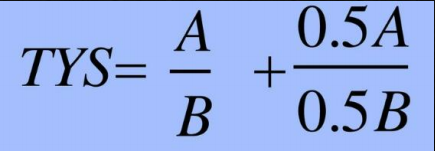
\includegraphics[width=0.8\textwidth]{images/shoe_tying_example.png}
 \caption{Computational Analysis of Shoe Tying: Application, Architecture, and Algorithm}
 \label{fig:shoe_tying_example}
\end{figure}

The seemingly simple act of tying a shoe provides an excellent introduction to computational thinking because it demonstrates how complex real-world activities can be broken down into computational components. Figure~\ref{fig:shoe_tying_example} illustrates how this everyday task exemplifies the three fundamental pillars of computational science.

\subsubsection{Application: What is the Science of Tying a Shoe?}

The \textbf{Application} component addresses the real-world problem or scientific domain being studied. In the case of shoe tying, this involves understanding the physical and biomechanical aspects of the task:

\begin{itemize}
    \item \textbf{Material Science}: Understanding the properties of shoelaces, including elasticity, friction coefficients, and durability under stress
    \item \textbf{Biomechanics}: Analyzing human finger dexterity, hand coordination, and motor control required for precise manipulation
    \item \textbf{Topology}: Studying the mathematical properties of knots and their stability under various loading conditions
    \item \textbf{Ergonomics}: Examining optimal techniques for efficient and comfortable shoe tying
    \item \textbf{Mechanical Engineering}: Understanding tension distribution, load-bearing capacity, and failure modes of different knot types
\end{itemize}

The scientific questions might include: What makes certain knots more secure than others? How do different lacing patterns affect foot comfort and support? What are the optimal materials for shoelaces in different environments?

\subsubsection{Architecture: A Computational Shoe}

The \textbf{Architecture} component represents the computational tools and environment needed to study and simulate the shoe tying process:

\begin{itemize}
    \item \textbf{Simulation Software}: Physics engines capable of modeling flexible materials and rope dynamics
    \item \textbf{3D Modeling Tools}: Computer-aided design software for creating detailed shoe and lace geometries
    \item \textbf{Motion Capture Systems}: Hardware for recording and analyzing human hand movements during shoe tying
    \item \textbf{Finite Element Analysis}: Computational tools for stress analysis and material deformation simulation
    \item \textbf{Virtual Reality Platforms}: Immersive environments for training and studying different tying techniques
    \item \textbf{Database Systems}: Storage and retrieval of experimental data, user studies, and performance metrics
\end{itemize}

The computational architecture must support real-time interaction, complex geometry manipulation, and detailed physics simulation to accurately represent the shoe tying process.

\subsubsection{Algorithm: Determining the Mathematics}

The \textbf{Algorithm} component involves the mathematical methods and computational procedures that transform the physical shoe tying process into solvable equations:

\textbf{Key Variables and Parameters:}
\begin{itemize}
    \item \textbf{Geometric Variables}: Lace length, shoe dimensions, eyelet positions, and spacing
    \item \textbf{Material Properties}: Young's modulus, friction coefficients, and tensile strength of laces
    \item \textbf{Force Variables}: Applied tensions, contact forces, and constraint forces at eyelets
    \item \textbf{Kinematic Variables}: Hand positions, velocities, and acceleration during the tying process
\end{itemize}

\textbf{Mathematical Assumptions and Models:}
\begin{itemize}
    \item \textbf{Flexible Body Dynamics}: Treating laces as continuous flexible cables with bending and torsional stiffness
    \item \textbf{Contact Mechanics}: Modeling friction and normal forces between laces and eyelets
    \item \textbf{Knot Theory}: Mathematical representation of different knot topologies and their properties
    \item \textbf{Optimization}: Finding optimal tying sequences that minimize effort while maximizing security
\end{itemize}

\textbf{The "TYS" Formula Example:}

The image shows a simplified mathematical relationship for "Tying Your Shoe" (TYS):

\begin{equation}
TYS = \frac{A}{B} + \frac{0.5A}{0.5B}
\end{equation}

Where:
\begin{itemize}
    \item $A$ represents factors that increase tying complexity (lace length, knot complexity, environmental conditions)
    \item $B$ represents factors that facilitate tying (user skill level, tool assistance, optimal technique)
\end{itemize}

This simplified model demonstrates how complex real-world processes can be abstracted into mathematical relationships that capture the essential factors influencing performance.

\subsubsection{Integration of the Three Pillars}

The shoe tying example demonstrates how the three pillars work synergistically:

\begin{itemize}
    \item \textbf{Application-Algorithm Interface}: Physical understanding of knot mechanics informs the mathematical models used in simulation
    \item \textbf{Algorithm-Architecture Interface}: Mathematical models determine the computational requirements and software design
    \item \textbf{Architecture-Application Interface}: Computational capabilities enable new types of experiments and studies not possible with manual methods alone
\end{itemize}

\subsection{Example 2: A Computational Geode}

\begin{figure}[h]
 \centering
 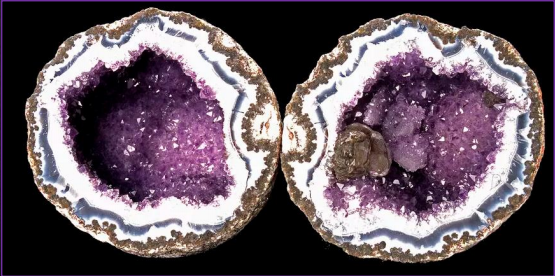
\includegraphics[width=0.8\textwidth]{images/computational_geode.png}
 \caption{Computational Analysis of Geode Formation: Application, Architecture, and Algorithm}
 \label{fig:computational_geode}
\end{figure}

Figure~\ref{fig:computational_geode} presents a more complex scientific example that illustrates how computational science approaches natural phenomena with extraordinary complexity and beauty. The formation of geodes represents a fascinating intersection of geology, chemistry, and physics that can only be fully understood through computational modeling.

\subsubsection{Application: The "Jewel" - Understanding Geode Formation}

The \textbf{Application} component focuses on the natural scientific phenomena that drive geode formation:

\begin{itemize}
    \item \textbf{Geological Processes}: Understanding how cavities form in host rocks through volcanic activity, sedimentary processes, or chemical dissolution
    \item \textbf{Crystallography}: Studying how different minerals nucleate and grow in confined spaces under varying conditions
    \item \textbf{Geochemistry}: Analyzing how mineral-rich solutions infiltrate cavities and precipitate crystals over geological time scales
    \item \textbf{Thermodynamics}: Understanding the energy relationships that drive crystal formation and determine final crystal structures
    \item \textbf{Fluid Dynamics}: Modeling how aqueous solutions move through porous rock and concentrate in geode cavities
\end{itemize}

The scientific questions include: What conditions lead to the formation of different crystal types within geodes? How do temperature, pressure, and chemical composition affect crystal growth patterns? What processes create the characteristic banded structures observed in many geodes?

\subsubsection{Architecture: The "Tool" - Computational Infrastructure}

The \textbf{Architecture} component encompasses the sophisticated computational tools required to model geological processes:

\begin{itemize}
    \item \textbf{High-Performance Computing Clusters}: Parallel processing systems capable of handling the massive computational demands of geological simulations
    \item \textbf{Geological Modeling Software}: Specialized applications for 3D geological visualization and subsurface modeling
    \item \textbf{Molecular Dynamics Simulators}: Tools for modeling atomic-scale crystal growth processes
    \item \textbf{Fluid Flow Simulation Software}: Computational fluid dynamics tools for modeling groundwater and hydrothermal fluid movement
    \item \textbf{Image Processing Systems}: Advanced visualization tools for creating detailed 3D renderings of geode structures
    \item \textbf{Database Management}: Systems for storing and analyzing vast datasets of geological, geochemical, and mineralogical information
\end{itemize}

\subsubsection{Algorithm: The "Rule" - Mathematical Frameworks}

The \textbf{Algorithm} component involves the complex mathematical and computational methods needed to simulate geode formation:

\textbf{Multi-Scale Modeling Approaches:}
\begin{itemize}
    \item \textbf{Atomic Scale}: Quantum mechanical calculations for crystal nucleation and surface energy calculations
    \item \textbf{Crystal Scale}: Kinetic Monte Carlo methods for simulating crystal growth processes
    \item \textbf{Cavity Scale}: Diffusion equations for solute transport and precipitation within geode cavities
    \item \textbf{Regional Scale}: Groundwater flow models and geological process simulation over thousands of years
\end{itemize}

\textbf{Key Mathematical Models:}
\begin{itemize}
    \item \textbf{Crystallization Kinetics}: Rate equations describing how crystals nucleate and grow from supersaturated solutions
    \item \textbf{Diffusion Equations}: Partial differential equations modeling how dissolved minerals move through solution
    \item \textbf{Thermodynamic Equilibrium}: Phase diagrams and chemical potential calculations determining stable mineral assemblages
    \item \textbf{Fracture Mechanics}: Models describing how initial cavities form and evolve in host rocks
\end{itemize}

\textbf{Computational Challenges:}
\begin{itemize}
    \item \textbf{Time Scale Integration}: Bridging processes occurring over microseconds (crystal growth) with geological time scales (millions of years)
    \item \textbf{Multi-Physics Coupling}: Integrating thermal, chemical, mechanical, and hydrological processes
    \item \textbf{Uncertainty Quantification}: Handling incomplete knowledge about ancient geological conditions
    \item \textbf{Validation}: Comparing computational predictions with observed geode structures and compositions
\end{itemize}

\subsubsection{The Scientific Impact}

The computational geode example demonstrates several key advantages of the computational science approach:

\begin{itemize}
    \item \textbf{Temporal Accessibility}: Simulating processes that occur over millions of years in reasonable computational time
    \item \textbf{Process Isolation}: Testing individual factors (temperature, pressure, chemistry) that cannot be controlled in natural settings
    \item \textbf{Predictive Capability}: Forecasting geode occurrence and characteristics for mineral exploration
    \item \textbf{Educational Value}: Creating visualizations that help students understand complex geological processes
\end{itemize}

\subsection{Comparative Analysis: Simple vs. Complex Applications}

\begin{examplecountercard}
\textbf{Simple System: Shoe Tying}
\begin{itemize}
    \item \textbf{Time Scale}: Seconds to minutes
    \item \textbf{Spatial Scale}: Centimeters to meters
    \item \textbf{Variables}: Dozens (forces, positions, materials)
    \item \textbf{Validation}: Direct observation and measurement
    \item \textbf{Applications}: Training, ergonomics, product design
\end{itemize}
\tcblower
\textbf{Complex System: Geode Formation}
\begin{itemize}
    \item \textbf{Time Scale}: Thousands to millions of years
    \item \textbf{Spatial Scale}: Atomic to regional scales
    \item \textbf{Variables}: Thousands (chemistry, temperature, pressure, time)
    \item \textbf{Validation}: Geological evidence, laboratory analogs
    \item \textbf{Applications}: Mineral exploration, geological education
\end{itemize}
\end{examplecountercard}

\subsection{Universal Principles Across Applications}

Despite the vast differences in complexity between shoe tying and geode formation, both examples demonstrate universal principles of computational science:

\subsubsection{Problem Decomposition}

Both problems benefit from breaking complex systems into manageable components:
\begin{itemize}
    \item \textbf{Hierarchical Structure}: Organizing problems from basic elements to complex assemblies
    \item \textbf{Interface Definition}: Clearly defining how components interact with each other
    \item \textbf{Modular Approach}: Developing solutions that can be tested and validated independently
\end{itemize}

\subsubsection{Mathematical Abstraction}

Both examples require translating physical phenomena into mathematical representations:
\begin{itemize}
    \item \textbf{Variable Identification}: Determining the key factors that influence system behavior
    \item \textbf{Relationship Modeling}: Establishing mathematical relationships between variables
    \item \textbf{Simplification Strategies}: Making appropriate assumptions to make problems tractable
\end{itemize}

\subsubsection{Computational Implementation}

Both problems require thoughtful selection of computational tools and methods:
\begin{itemize}
    \item \textbf{Scale Matching}: Choosing computational approaches appropriate for the spatial and temporal scales involved
    \item \textbf{Resource Optimization}: Balancing computational accuracy with available resources
    \item \textbf{Validation Strategies}: Developing methods to verify that computational results represent reality accurately
\end{itemize}

\subsubsection{Interdisciplinary Integration}

Both examples demonstrate the need for knowledge from multiple domains:
\begin{itemize}
    \item \textbf{Domain Expertise}: Deep understanding of the physical phenomena being modeled
    \item \textbf{Mathematical Modeling}: Ability to translate phenomena into mathematical form
    \item \textbf{Computational Skills}: Technical expertise in implementing and running computational models
\end{itemize}

\subsection{Learning Progression: From Simple to Complex}

The contrast between these examples illustrates an important pedagogical principle in computational science education:

\begin{highlightbox}{Educational Scaffolding}
\textbf{Starting with Simple, Familiar Examples} like shoe tying helps students understand the fundamental concepts of computational thinking without being overwhelmed by domain-specific complexity. Once these concepts are mastered, students can progress to \textbf{Complex Scientific Applications} like geode formation that demonstrate the full power and potential of computational science approaches.
\end{highlightbox}

This progression helps students develop:
\begin{itemize}
    \item \textbf{Confidence}: Building skills on accessible problems before tackling complex scientific challenges
    \item \textbf{Intuition}: Developing an understanding of when and how to apply computational approaches
    \item \textbf{Perspective}: Appreciating the wide range of problems that can benefit from computational analysis
    \item \textbf{Skills Transfer}: Learning to apply computational thinking across diverse domains
\end{itemize}

The examples of shoe tying and geode formation thus serve as bookends for the spectrum of computational science applications—from the everyday and accessible to the scientifically profound and complex. Both demonstrate that computational science is fundamentally about understanding systems through the integration of real-world knowledge, mathematical modeling, and computational implementation.

\section{What Computational Science is NOT!}

\begin{warningbox}{Common Misconceptions}
While understanding what computational science \textbf{is} provides crucial foundation, it is equally important to clarify what computational science is \textbf{NOT}. Many students and professionals mistakenly equate computational science with basic computer usage or simple data manipulation tasks. This section addresses these misconceptions to establish clear boundaries and expectations.
\end{warningbox}

One of the most persistent challenges in computational science education is addressing common misconceptions about the field's scope and purpose. Many students entering computational science courses bring preconceived notions based on their prior experiences with computers, data analysis, or programming. While these experiences may be valuable, they often represent only superficial aspects of what computational science truly encompasses.

The distinction between computational science and routine computer usage is fundamental to understanding the field's unique contributions to scientific discovery. Computational science is not simply about using computers as tools—it is about employing computational thinking to solve complex scientific problems through the integration of domain knowledge, mathematical modeling, and sophisticated computational methods.

\subsection{Computational Science vs. Basic Data Management}

\subsubsection{Putting Numbers into Spreadsheets}

\begin{conceptcard}{Not Computational Science: Spreadsheet Data Entry}
Simply entering numerical data into spreadsheet applications like Microsoft Excel, Google Sheets, or similar software does \textbf{not} constitute computational science. While spreadsheets can be valuable tools for organizing and presenting data, the mere act of data entry lacks the analytical depth, mathematical modeling, and scientific reasoning that define computational science.
\end{conceptcard}

Basic spreadsheet usage typically involves:
\begin{itemize}
    \item Manual data entry from external sources
    \item Simple arithmetic calculations using built-in functions
    \item Basic formatting and organization of tabular data
    \item Creation of simple charts and graphs for presentation
    \item Data storage and retrieval without advanced analysis
\end{itemize}

\textbf{Why This Falls Short of Computational Science:}
\begin{itemize}
    \item \textbf{Lack of Mathematical Modeling}: Spreadsheets typically handle existing data without developing mathematical relationships or predictive models
    \item \textbf{Limited Scientific Integration}: Data entry focuses on organization rather than understanding underlying scientific phenomena
    \item \textbf{Absence of Computational Thinking}: The process involves mechanical tasks rather than algorithmic problem-solving approaches
    \item \textbf{No Hypothesis Testing}: Simple data organization does not involve formulating and testing scientific hypotheses
    \item \textbf{Minimal Analytical Depth}: Basic spreadsheet operations lack the sophisticated analysis required for scientific discovery
\end{itemize}

\textbf{When Spreadsheets Can Support Computational Science:}
While basic spreadsheet usage is not computational science, spreadsheets can serve as components within larger computational science workflows:
\begin{itemize}
    \item Preliminary data exploration and visualization
    \item Simple model prototyping and parameter studies
    \item Data preparation for more sophisticated analysis tools
    \item Communication of results to non-technical audiences
    \item Educational demonstrations of basic computational concepts
\end{itemize}

\subsubsection{Analyzing Data Gathered in the Field or Experimentally}

\begin{conceptcard}{Not Computational Science: Basic Data Analysis}
While data analysis is an important scientific skill, routine analysis of experimental or field data using standard statistical methods does \textbf{not} automatically qualify as computational science. The key distinction lies in the depth of integration between domain science, mathematical modeling, and computational methodology.
\end{conceptcard}

Traditional data analysis typically includes:
\begin{itemize}
    \item Descriptive statistics (means, standard deviations, distributions)
    \item Standard statistical tests (t-tests, ANOVA, correlation analysis)
    \item Basic regression analysis using established methods
    \item Data visualization through standard plotting techniques
    \item Quality control and error checking of datasets
\end{itemize}

\textbf{Limitations of Basic Data Analysis:}
\begin{itemize}
    \item \textbf{Reactive Rather Than Predictive}: Traditional analysis describes what has been observed rather than predicting future behavior
    \item \textbf{Limited Model Development}: Standard statistical methods apply existing techniques rather than developing new mathematical models
    \item \textbf{Narrow Scope}: Analysis often focuses on specific datasets without broader scientific integration
    \item \textbf{Tool-Driven Rather Than Problem-Driven}: The choice of analysis method may be limited by available software rather than scientific requirements
    \item \textbf{Insufficient Theoretical Integration}: Analysis may lack connection to underlying scientific theory and principles
\end{itemize}

\textbf{Transition to Computational Science:}
Data analysis becomes computational science when it incorporates:
\begin{itemize}
    \item Development of mathematical models that explain observed phenomena
    \item Integration of multiple datasets to test comprehensive hypotheses
    \item Creation of predictive models that can forecast future states
    \item Coupling of data analysis with theoretical understanding
    \item Design of computational experiments to explore parameter spaces
\end{itemize}

\subsection{Computational Science vs. Simple Mathematical Operations}

\subsubsection{Fitting Data to an Equation}

\begin{conceptcard}{Not Computational Science: Curve Fitting}
Using software to fit experimental data to predetermined mathematical functions (such as linear, polynomial, or exponential curves) represents curve fitting rather than computational science. While curve fitting can be a component of computational science, it alone lacks the comprehensive approach that characterizes the field.
\end{conceptcard}

Standard curve fitting involves:
\begin{itemize}
    \item Selecting from a library of common mathematical functions
    \item Using software to minimize residual errors between data and function
    \item Evaluating goodness-of-fit statistics (R-squared, residual analysis)
    \item Extracting parameter values from the fitted function
    \item Using fitted equations for interpolation within the data range
\end{itemize}

\textbf{Why Curve Fitting Alone Is Insufficient:}
\begin{itemize}
    \item \textbf{Lacks Scientific Justification}: Function selection may be based on mathematical convenience rather than physical understanding
    \item \textbf{Limited Predictive Power}: Fitted curves may not extrapolate reliably beyond the original data range
    \item \textbf{Absence of Mechanism}: Fitting does not necessarily reveal the underlying processes that generate the observed behavior
    \item \textbf{Statistical Rather Than Scientific}: Focus on mathematical fit rather than scientific insight
    \item \textbf{Tool-Dependent}: Results may vary significantly based on the specific software or algorithm used
\end{itemize}

\textbf{Computational Science Approach to Mathematical Modeling:}
Curve fitting becomes part of computational science when it includes:
\begin{itemize}
    \item Derivation of mathematical models from first principles
    \item Integration of multiple physical processes in comprehensive models
    \item Validation of models against independent datasets
    \item Use of models to explore scenarios beyond experimental conditions
    \item Incorporation of uncertainty quantification and sensitivity analysis
\end{itemize}

\subsubsection{Visualizing Data Collected Experimentally or in the Field}

\begin{conceptcard}{Not Computational Science: Basic Data Visualization}
Creating charts, graphs, and plots from experimental or field data using standard software tools constitutes data visualization rather than computational science. While effective visualization is important for scientific communication, it represents only one aspect of the broader computational science methodology.
\end{conceptcard}

Standard data visualization includes:
\begin{itemize}
    \item Creating scatter plots, bar charts, and line graphs
    \item Generating histograms and distribution plots
    \item Producing basic 3D surface plots and contour maps
    \item Adding trend lines and error bars to plots
    \item Formatting plots for presentations and publications
\end{itemize}

\textbf{Limitations of Basic Visualization:}
\begin{itemize}
    \item \textbf{Descriptive Rather Than Explanatory}: Plots show data patterns without explaining underlying mechanisms
    \item \textbf{Static Rather Than Interactive}: Traditional plots cannot explore dynamic relationships or parameter variations
    \item \textbf{Limited Dimensionality}: Standard plots struggle to represent complex, multi-dimensional relationships
    \item \textbf{No Model Integration}: Visualization may be disconnected from mathematical models or theoretical understanding
    \item \textbf{Presentation-Focused}: Emphasis on communication rather than scientific discovery
\end{itemize}

\textbf{Scientific Visualization in Computational Science:}
Visualization becomes computational science when it enables:
\begin{itemize}
    \item Interactive exploration of high-dimensional parameter spaces
    \item Real-time visualization of dynamic simulations and models
    \item Integration of multiple data sources and model predictions
    \item Discovery of unexpected patterns and relationships
    \item Communication of complex scientific concepts and findings
\end{itemize}

\subsection{Computational Science vs. General Computing Tasks}

\subsubsection{Writing a Computer Program}

\begin{conceptcard}{Not Computational Science: General Programming}
Simply writing computer programs or software applications does \textbf{not} constitute computational science. While programming skills are essential tools for computational scientists, the act of coding itself must be directed toward solving scientific problems through mathematical modeling and computational analysis.
\end{conceptcard}

General programming activities include:
\begin{itemize}
    \item Learning programming languages and syntax
    \item Developing user interfaces and web applications
    \item Creating databases and information management systems
    \item Building general-purpose software tools and utilities
    \item Implementing standard algorithms and data structures
\end{itemize}

\textbf{Distinguishing Programming from Computational Science:}
\begin{itemize}
    \item \textbf{Purpose}: General programming serves diverse applications; computational science programming specifically targets scientific problem-solving
    \item \textbf{Domain Integration}: Computational science programming requires deep understanding of the scientific domain being studied
    \item \textbf{Mathematical Foundation}: Scientific programming implements mathematical models and numerical methods rather than general algorithms
    \item \textbf{Validation Requirements}: Scientific code must be validated against theoretical predictions and experimental data
    \item \textbf{Interdisciplinary Context}: Computational science programming operates at the intersection of domain science, mathematics, and computing
\end{itemize}

\textbf{Scientific Programming Characteristics:}
Programming becomes computational science when it involves:
\begin{itemize}
    \item Implementation of mathematical models derived from scientific theory
    \item Development of numerical methods for solving scientific problems
    \item Integration of multiple physical processes and scales
    \item Validation and verification against experimental data
    \item Optimization for high-performance scientific computing
\end{itemize}

\subsubsection{Using a Computer for Databases, Word Processing, or Presentations}

\begin{conceptcard}{Not Computational Science: Office Applications}
Using computers for general productivity tasks such as database management, word processing, or presentation creation represents routine computer usage rather than computational science. These activities, while potentially supporting scientific work, lack the analytical and modeling components that define computational science.
\end{conceptcard}

Standard office computing includes:
\begin{itemize}
    \item Creating and maintaining databases for record-keeping
    \item Writing reports, papers, and documentation
    \item Developing presentations for meetings and conferences
    \item Managing email communication and file organization
    \item Using standard business software for administrative tasks
\end{itemize}

\textbf{Why Office Applications Are Not Computational Science:}
\begin{itemize}
    \item \textbf{Administrative Rather Than Analytical}: Focus on information management rather than scientific discovery
    \item \textbf{No Mathematical Modeling}: Activities do not involve developing or implementing mathematical relationships
    \item \textbf{Limited Scientific Integration}: Tasks are disconnected from scientific theory and methodology
    \item \textbf{Tool Usage Rather Than Tool Development}: Using existing software rather than creating new computational approaches
    \item \textbf{Communication Rather Than Investigation}: Emphasis on presenting information rather than generating new knowledge
\end{itemize}

\textbf{Supporting Role in Computational Science:}
Office applications can support computational science through:
\begin{itemize}
    \item Documentation of computational methods and results
    \item Communication of scientific findings to diverse audiences
    \item Management of computational workflows and project data
    \item Collaboration among interdisciplinary research teams
    \item Integration of computational results with broader scientific communication
\end{itemize}

\subsection{The Integration Imperative: What Makes It Computational Science}

\begin{highlightbox}{The Computational Science Difference}
The key distinction is not in the individual activities but in their \textbf{integration and purpose}. Computational science emerges when computer usage is guided by scientific questions, informed by mathematical modeling, and directed toward understanding complex phenomena that cannot be adequately addressed through traditional experimental or theoretical approaches alone.
\end{highlightbox}

\subsubsection{Essential Components for Computational Science}

For any computational activity to qualify as computational science, it must integrate:

\textbf{1. Scientific Purpose and Context}
\begin{itemize}
    \item Clear scientific questions driving the computational investigation
    \item Understanding of relevant physical, biological, or social phenomena
    \item Connection to broader scientific knowledge and theory
    \item Potential for advancing scientific understanding or capability
\end{itemize}

\textbf{2. Mathematical Foundation}
\begin{itemize}
    \item Mathematical models that represent key aspects of the scientific system
    \item Quantitative relationships between variables and parameters
    \item Theoretical framework linking mathematical description to physical reality
    \item Appropriate mathematical methods for the scientific domain
\end{itemize}

\textbf{3. Computational Implementation}
\begin{itemize}
    \item Algorithms and numerical methods suited to the scientific problem
    \item Software implementation that efficiently solves the mathematical model
    \item Appropriate computational architecture for the problem scale
    \item Validation and verification of computational results
\end{itemize}

\textbf{4. Scientific Validation and Interpretation}
\begin{itemize}
    \item Comparison of computational results with experimental data
    \item Assessment of model limitations and uncertainties
    \item Scientific interpretation of computational findings
    \item Contribution to scientific knowledge and understanding
\end{itemize}

\subsubsection{From Basic Computing to Computational Science}

The transition from basic computer usage to computational science involves several levels of increasing sophistication:

\textbf{Level 1: Basic Computer Literacy}
\begin{itemize}
    \item Using computers for general productivity tasks
    \item Basic data entry and simple calculations
    \item Standard software applications and file management
\end{itemize}

\textbf{Level 2: Data Analysis and Visualization}
\begin{itemize}
    \item Statistical analysis of experimental data
    \item Creation of scientific plots and charts
    \item Simple mathematical modeling and curve fitting
\end{itemize}

\textbf{Level 3: Scientific Programming}
\begin{itemize}
    \item Custom software development for scientific applications
    \item Implementation of mathematical models and algorithms
    \item Integration of multiple data sources and analysis methods
\end{itemize}

\textbf{Level 4: Computational Science}
\begin{itemize}
    \item Integration of domain science, mathematics, and computing
    \item Development of new computational methods for scientific problems
    \item Validation of computational models against scientific theory and experiment
    \item Contribution to scientific discovery and understanding
\end{itemize}

\subsection{Educational Implications}

Understanding what computational science is not helps establish appropriate expectations and learning objectives for students entering the field. This clarity is essential for:

\begin{itemize}
    \item \textbf{Curriculum Design}: Ensuring courses progress beyond basic computer usage toward true computational science
    \item \textbf{Student Preparation}: Helping students understand the interdisciplinary nature and depth of computational science
    \item \textbf{Assessment Criteria}: Evaluating student work based on computational science principles rather than basic computer skills
    \item \textbf{Career Guidance}: Preparing students for roles that require genuine computational science expertise
    \item \textbf{Research Expectations}: Establishing standards for computational science research and scholarship
\end{itemize}

By clearly distinguishing computational science from basic computer usage, students can better appreciate the field's unique contributions and develop the comprehensive skills necessary for success in computational science careers and research.

\section{Why Do We Need Computational Science?}

\begin{conceptcard}{The Necessity of Computational Science}
Computational science has emerged as an essential discipline because there are many fascinating and important problems that \textbf{cannot be solved} using traditional experimental or theoretical methods alone. These problems require the unique capabilities that computational approaches provide, bridging gaps where conventional methods fall short.
\end{conceptcard}

The question ``Why do we need computational science?'' strikes at the heart of the field's value proposition and relevance to modern scientific inquiry. The answer lies not in computational science being merely a convenient alternative to traditional methods, but in its ability to address fundamental limitations that restrict our capacity to understand and solve complex problems.

In many scientific domains, researchers encounter scenarios where traditional approaches—whether experimental investigation or theoretical analysis—prove inadequate, impractical, or impossible. Computational science provides the tools and methodologies necessary to tackle these challenging problems, opening new frontiers for scientific discovery and technological advancement.

\subsection{Limitations of Traditional Methods}

\subsubsection{Problems Too Tedious for Manual Calculation}

\begin{warningbox}{The Tedium Barrier}
Many scientifically important problems involve calculations that are \textbf{too tedious} to solve using calculators or manual computation. These problems may be theoretically solvable but practically impossible due to the sheer volume of arithmetic operations required.
\end{warningbox}

Manual calculation becomes prohibitively tedious when problems involve:

\textbf{Massive Scale Computations:}
\begin{itemize}
    \item \textbf{Weather Prediction}: Calculating atmospheric conditions across millions of grid points requires billions of mathematical operations updated every few minutes
    \item \textbf{Structural Analysis}: Determining stress and strain in complex engineering structures involves solving systems with hundreds of thousands of equations
    \item \textbf{Financial Modeling}: Risk assessment for large investment portfolios requires evaluating thousands of scenarios with multiple variables
    \item \textbf{Genomic Analysis}: Processing DNA sequences with millions of base pairs demands computational power far beyond manual calculation
\end{itemize}

\textbf{Iterative Processes:}
\begin{itemize}
    \item \textbf{Optimization Problems}: Finding optimal solutions often requires testing thousands or millions of parameter combinations
    \item \textbf{Numerical Integration}: Accurate integration of complex functions may require millions of calculation steps
    \item \textbf{Convergence Algorithms}: Many mathematical methods require repeated iterations until convergence criteria are met
    \item \textbf{Monte Carlo Simulations}: Statistical accuracy requires running simulations thousands or millions of times
\end{itemize}

\textbf{Real-Time Requirements:}
\begin{itemize}
    \item \textbf{Navigation Systems}: GPS calculations must be completed in milliseconds to provide useful location information
    \item \textbf{Medical Imaging}: CT scans and MRI processing require immediate reconstruction of images from raw data
    \item \textbf{Industrial Control}: Manufacturing processes need instantaneous feedback and adjustment
    \item \textbf{Financial Trading}: Market analysis and trading decisions must occur faster than human reaction times
\end{itemize}

\subsubsection{Problems Too Dangerous for Laboratory Investigation}

\begin{warningbox}{The Safety Imperative}
Certain scientific questions involve phenomena that are \textbf{too dangerous} to investigate through direct laboratory experimentation. Computational science provides a safe virtual laboratory for exploring these hazardous scenarios without risking human safety or environmental damage.
\end{warningbox}

Dangerous scenarios that require computational investigation include:

\textbf{Nuclear and Radioactive Phenomena:}
\begin{itemize}
    \item \textbf{Nuclear Reactor Safety}: Testing reactor failure scenarios computationally prevents potential catastrophic accidents
    \item \textbf{Nuclear Weapons Research}: Computer simulations replace underground testing, reducing environmental contamination
    \item \textbf{Radioactive Waste Management}: Modeling long-term radioactive decay and containment without exposing researchers to radiation
    \item \textbf{Medical Radiation Therapy}: Optimizing treatment protocols without exposing patients to experimental doses
\end{itemize}

\textbf{Extreme Environmental Conditions:}
\begin{itemize}
    \item \textbf{Volcanic Eruptions}: Studying eruption dynamics and lava flows without risking lives near active volcanoes
    \item \textbf{Hurricane and Tornado Formation}: Investigating storm dynamics without flying aircraft into dangerous weather
    \item \textbf{Deep Ocean Exploration}: Modeling underwater volcanic activity and pressure effects without risking submersibles
    \item \textbf{Space Weather}: Understanding solar flare impacts without exposing spacecraft and astronauts to harmful radiation
\end{itemize}

\textbf{Chemical and Biological Hazards:}
\begin{itemize}
    \item \textbf{Toxic Chemical Reactions}: Studying dangerous chemical processes without creating hazardous waste or exposing researchers
    \item \textbf{Infectious Disease Modeling}: Understanding pandemic spread without deliberately exposing populations to pathogens
    \item \textbf{Explosive Materials}: Testing energetic materials and explosives computationally for safety applications
    \item \textbf{Environmental Contamination}: Modeling pollution effects without actually contaminating ecosystems
\end{itemize}

\subsubsection{Problems Too Expensive for Physical Implementation}

\begin{warningbox}{The Economic Reality}
Many important scientific and engineering problems are \textbf{too expensive} to investigate through physical experimentation. Computational science offers cost-effective alternatives that provide valuable insights without the enormous financial investments required for large-scale physical testing.
\end{warningbox}

Economically prohibitive investigations include:

\textbf{Large-Scale Engineering Projects:}
\begin{itemize}
    \item \textbf{Aircraft Design}: Building and testing multiple aircraft prototypes costs billions of dollars; computational fluid dynamics reduces the need for physical prototypes
    \item \textbf{Bridge and Building Construction}: Testing structural designs computationally prevents costly construction failures
    \item \textbf{Automotive Safety}: Crash testing every possible scenario would require thousands of vehicles; computer simulations test safety features efficiently
    \item \textbf{Space Mission Planning}: Computational modeling validates mission designs before committing billions to spacecraft construction
\end{itemize}

\textbf{Pharmaceutical Development:}
\begin{itemize}
    \item \textbf{Drug Discovery}: Computational screening of millions of molecular compounds reduces the need for expensive laboratory synthesis
    \item \textbf{Clinical Trial Design}: Modeling patient responses helps optimize trial protocols, reducing costs and patient risk
    \item \textbf{Drug Interaction Studies}: Computational pharmacology predicts drug interactions without extensive clinical testing
    \item \textbf{Personalized Medicine}: Modeling individual genetic variations computationally enables customized treatment approaches
\end{itemize}

\textbf{Environmental and Climate Studies:}
\begin{itemize}
    \item \textbf{Climate Change Research}: Creating multiple Earth-like planets for controlled climate experiments is impossible; computational models provide the only feasible approach
    \item \textbf{Ecosystem Management}: Testing different conservation strategies across entire ecosystems computationally before implementation
    \item \textbf{Resource Exploration}: Computational modeling reduces the cost of unsuccessful oil, gas, and mineral exploration
    \item \textbf{Agricultural Optimization}: Testing crop varieties and farming techniques computationally before large-scale field trials
\end{itemize}

\subsubsection{Problems Solvable Only Through Mathematical and Computational Tools}

\begin{conceptcard}{Computational-Only Solutions}
Some problems are fundamentally \textbf{solvable only} through mathematical techniques and computational tools. These problems involve phenomena that cannot be directly observed, manipulated, or replicated in laboratory settings, making computational approaches the sole viable method for investigation.
\end{conceptcard}

Computational-only problems include:

\textbf{Temporal Scale Challenges:}
\begin{itemize}
    \item \textbf{Geological Processes}: Understanding mountain formation, continental drift, and geological evolution over millions of years
    \item \textbf{Stellar Evolution}: Modeling the birth, life, and death of stars across billions of years
    \item \textbf{Archaeological Reconstruction}: Recreating ancient civilizations and historical events from limited evidence
    \item \textbf{Evolutionary Biology}: Tracing species evolution and genetic changes across millennia
\end{itemize}

\textbf{Spatial Scale Extremes:}
\begin{itemize}
    \item \textbf{Quantum Mechanics}: Modeling subatomic particle behavior and quantum systems that cannot be directly observed
    \item \textbf{Cosmological Phenomena}: Understanding the formation and evolution of galaxies, black holes, and the universe itself
    \item \textbf{Molecular Dynamics}: Studying protein folding and molecular interactions at atomic scales
    \item \textbf{Nanotechnology}: Designing and testing nanoscale devices and materials
\end{itemize}

\textbf{Abstract Mathematical Concepts:}
\begin{itemize}
    \item \textbf{Complex System Behavior}: Understanding emergent properties in systems with many interacting components
    \item \textbf{Chaos Theory}: Exploring sensitive dependence on initial conditions in nonlinear systems
    \item \textbf{Network Analysis}: Modeling complex networks like the internet, social networks, and neural networks
    \item \textbf{Information Theory}: Analyzing data compression, encryption, and communication systems
\end{itemize}

\subsection{The Marriage of Mathematics, Computing, and Science}

\begin{highlightbox}{Interdisciplinary Synthesis}
Computational science establishes a \textbf{true marriage} between mathematics, computing, and science. This integration creates capabilities that exceed what any single discipline could achieve independently, enabling solutions to problems that would otherwise remain unsolvable.
\end{highlightbox}

\subsubsection{Mathematics Provides the Language}

Mathematics serves as the universal language that describes natural phenomena:
\begin{itemize}
    \item \textbf{Differential Equations}: Describe rates of change and dynamic processes
    \item \textbf{Linear Algebra}: Handles multi-dimensional relationships and transformations
    \item \textbf{Statistics and Probability}: Manages uncertainty and variability in complex systems
    \item \textbf{Optimization Theory}: Finds best solutions among many possibilities
    \item \textbf{Graph Theory}: Models networks and relationships between entities
\end{itemize}

\subsubsection{Computing Provides the Power}

Computing contributes the computational power and tools necessary for implementation:
\begin{itemize}
    \item \textbf{Algorithmic Thinking}: Systematic approaches to problem-solving
    \item \textbf{Numerical Methods}: Techniques for solving mathematical problems computationally
    \item \textbf{High-Performance Computing}: Massive computational resources for large-scale problems
    \item \textbf{Software Engineering}: Robust, reliable, and maintainable computational tools
    \item \textbf{Data Management}: Efficient storage, retrieval, and processing of large datasets
\end{itemize}

\subsubsection{Science Provides the Context and Validation}

Science contributes domain knowledge and validation criteria:
\begin{itemize}
    \item \textbf{Physical Understanding}: Knowledge of natural laws and phenomena
    \item \textbf{Experimental Data}: Information for model validation and parameter estimation
    \item \textbf{Scientific Method}: Systematic approaches to hypothesis testing and theory development
    \item \textbf{Domain Expertise}: Deep understanding of specific scientific fields and applications
    \item \textbf{Quality Assurance}: Standards for evaluating the accuracy and reliability of computational results
\end{itemize}

\subsection{Who Cares? The Stakeholders and Beneficiaries}

\begin{conceptcard}{Universal Relevance}
The question ``Who cares?'' about computational science reveals the broad spectrum of stakeholders who benefit from computational approaches. The answer encompasses virtually every sector of society, from individual researchers to global organizations addressing humanity's greatest challenges.
\end{conceptcard}

\subsubsection{Academic and Research Communities}

\textbf{Universities and Research Institutions:}
\begin{itemize}
    \item Faculty researchers across all scientific disciplines rely on computational methods
    \item Graduate students require computational skills for thesis research and career preparation
    \item Undergraduate education increasingly incorporates computational thinking and methods
    \item Research funding agencies prioritize proposals that include computational components
\end{itemize}

\textbf{National Laboratories and Government Research:}
\begin{itemize}
    \item National security applications require advanced computational modeling
    \item Environmental monitoring and climate research depend on computational models
    \item Energy research and development relies heavily on computational simulation
    \item Public health and epidemiological studies use computational approaches
\end{itemize}

\subsubsection{Industry and Technology Sectors}

\textbf{Technology Companies:}
\begin{itemize}
    \item Software and hardware companies develop computational tools and platforms
    \item Data analytics and artificial intelligence companies rely on computational science foundations
    \item Technology consulting firms provide computational solutions to other industries
    \item Startups often build businesses around novel computational approaches
\end{itemize}

\textbf{Traditional Industries:}
\begin{itemize}
    \item Pharmaceutical companies use computational drug discovery and development
    \item Automotive and aerospace industries depend on computational design and testing
    \item Financial services rely on computational risk assessment and trading algorithms
    \item Manufacturing companies optimize production processes through computational modeling
\end{itemize}

\subsubsection{Society and Global Challenges}

\textbf{Healthcare and Medicine:}
\begin{itemize}
    \item Patients benefit from computationally-designed treatments and medical devices
    \item Healthcare providers use computational tools for diagnosis and treatment planning
    \item Public health officials rely on computational models for disease surveillance and prevention
    \item Medical researchers use computational approaches to understand disease mechanisms
\end{itemize}

\textbf{Environmental and Climate Issues:}
\begin{itemize}
    \item Policymakers rely on computational climate models for environmental decisions
    \item Conservation organizations use computational tools for ecosystem management
    \item Agricultural communities benefit from computationally-optimized farming practices
    \item Communities worldwide depend on computational weather prediction and natural disaster modeling
\end{itemize}

\textbf{Economic and Social Systems:}
\begin{itemize}
    \item Governments use computational models for economic planning and policy analysis
    \item Urban planners rely on computational tools for city design and traffic management
    \item Educational systems benefit from computationally-enhanced learning and assessment
    \item Social scientists use computational approaches to understand human behavior and social systems
\end{itemize}

\subsection{The Compelling Case for Computational Science}

The convergence of these factors—tedious calculations, dangerous experiments, expensive investigations, and unsolvable problems—creates a compelling case for computational science as an essential component of modern scientific and technological advancement. Computational science is not merely a convenience or alternative approach; it is often the only viable path forward for addressing humanity's most pressing challenges and advancing our understanding of the natural world.

\begin{examplebox}{Real-World Impact}
Consider the development of COVID-19 vaccines: Computational modeling accelerated the identification of viral protein structures, predicted vaccine effectiveness, and optimized manufacturing processes. Without computational science, vaccine development would have taken many years longer, potentially costing millions of additional lives. This example illustrates how computational science directly benefits society by enabling solutions that would be impossible through traditional methods alone.
\end{examplebox}

As we face increasingly complex global challenges—from climate change and pandemic preparedness to sustainable energy and space exploration—the need for computational science continues to grow. The field's ability to bridge traditional disciplinary boundaries and provide innovative solutions to previously intractable problems makes it indispensable for scientific progress and societal advancement in the 21st century and beyond.

\section{The Grand Challenges and Opportunities}

\begin{conceptcard}{21st Century Science: The Grand Challenges}
The 21st century presents humanity with unprecedented scientific challenges that require the full power of computational science. These grand challenges represent not just problems to be solved, but opportunities for transformative discoveries that could reshape our understanding of the world and our place in it.
\end{conceptcard}

\subsection{The Seven Grand Challenges of 21st Century Science}

The National Science Foundation and other leading scientific organizations have identified several grand challenges that define the frontiers of 21st century science. These challenges represent areas where computational science is not just helpful, but absolutely essential for progress.

\subsubsection{Molecular and Structural Biology}

\begin{highlightbox}{Understanding Life at the Molecular Level}
The quest to understand how biological systems work at the molecular level represents one of the most promising frontiers in science. Computational approaches are revolutionizing our ability to model protein structures, predict drug interactions, and design new therapeutic approaches.
\end{highlightbox}

\textbf{Key Computational Challenges:}
\begin{itemize}
    \item \textbf{Protein Folding Prediction}: Understanding how amino acid sequences fold into functional three-dimensional structures
    \item \textbf{Drug Discovery and Design}: Computationally screening millions of molecular compounds to identify potential medicines
    \item \textbf{Genomic Analysis}: Processing and interpreting vast amounts of genetic data to understand disease mechanisms
    \item \textbf{Systems Biology}: Modeling complex interactions between genes, proteins, and cellular processes
\end{itemize}

\textbf{Computational Impact:}
Recent breakthroughs like AlphaFold's protein structure prediction demonstrate how computational science can solve problems that have puzzled scientists for decades, opening new possibilities for understanding diseases and developing treatments.

\subsubsection{Cosmology and Fundamental Physics}

\begin{highlightbox}{Unraveling the Mysteries of the Universe}
Understanding the origin, evolution, and ultimate fate of the universe requires computational models that can simulate billions of years of cosmic evolution and probe the fundamental nature of matter, energy, space, and time.
\end{highlightbox}

\textbf{Key Computational Challenges:}
\begin{itemize}
    \item \textbf{Dark Matter and Dark Energy}: Modeling the mysterious components that comprise 95\% of the universe
    \item \textbf{Galaxy Formation and Evolution}: Simulating how structures formed in the early universe
    \item \textbf{Gravitational Waves}: Analyzing signals from cosmic events like black hole mergers
    \item \textbf{Quantum Gravity}: Developing theories that unify general relativity and quantum mechanics
\end{itemize}

\textbf{Computational Requirements:}
These problems require some of the most powerful supercomputers ever built, with simulations that can run for months and generate petabytes of data.

\subsubsection{Environmental Hydrology and Climate Science}

\begin{highlightbox}{Predicting and Managing Earth's Future}
Understanding Earth's climate system and water cycle is crucial for addressing climate change, managing water resources, and preparing for environmental challenges that will affect billions of people.
\end{highlightbox}

\textbf{Key Computational Challenges:}
\begin{itemize}
    \item \textbf{Climate Modeling}: Predicting future climate conditions under different scenarios
    \item \textbf{Water Resource Management}: Modeling groundwater, river systems, and ocean circulation
    \item \textbf{Extreme Weather Prediction}: Improving forecasts of hurricanes, droughts, and floods
    \item \textbf{Ecosystem Modeling}: Understanding how environmental changes affect biodiversity
\end{itemize}

\textbf{Societal Impact:}
Computational climate and environmental models directly inform policy decisions that affect the lives of billions of people and the future habitability of our planet.

\subsubsection{Warfare and Survivability}

\begin{highlightbox}{National Security in the Computational Age}
Modern national security depends increasingly on computational capabilities, from cybersecurity and autonomous systems to modeling complex geopolitical scenarios and protecting critical infrastructure.
\end{highlightbox}

\textbf{Key Computational Challenges:}
\begin{itemize}
    \item \textbf{Cybersecurity}: Protecting digital infrastructure from increasingly sophisticated attacks
    \item \textbf{Autonomous Systems}: Developing reliable AI for defense and security applications
    \item \textbf{Strategic Planning}: Modeling complex scenarios for national security decision-making
    \item \textbf{Critical Infrastructure Protection}: Ensuring resilience of power grids, communication networks, and transportation systems
\end{itemize}

\textbf{Ethical Considerations:}
This field raises important questions about the responsible development and deployment of computational technologies for security applications.

\subsubsection{Chemical Engineering and Molecular Structure}

\begin{highlightbox}{Designing Materials and Processes for the Future}
Computational chemistry and materials science are enabling the design of new materials with unprecedented properties, from superconductors and catalysts to advanced composites and nanomaterials.
\end{highlightbox}

\textbf{Key Computational Challenges:}
\begin{itemize}
    \item \textbf{Catalyst Design}: Developing more efficient catalysts for chemical processes and clean energy
    \item \textbf{Materials Discovery}: Predicting properties of new materials before they are synthesized
    \item \textbf{Process Optimization}: Improving efficiency and reducing waste in chemical manufacturing
    \item \textbf{Molecular Electronics}: Designing electronic devices at the molecular scale
\end{itemize}

\textbf{Industrial Impact:}
These advances are crucial for developing sustainable technologies, improving energy efficiency, and creating new industries based on advanced materials.

\subsubsection{Weather Prediction and Atmospheric Science}

\begin{highlightbox}{Mastering Earth's Atmosphere}
Accurate weather prediction remains one of the most computationally demanding and socially important applications of computational science, with implications for agriculture, transportation, energy, and public safety.
\end{highlightbox}

\textbf{Key Computational Challenges:}
\begin{itemize}
    \item \textbf{High-Resolution Weather Models}: Increasing spatial and temporal resolution of forecasts
    \item \textbf{Ensemble Forecasting}: Quantifying uncertainty in weather predictions
    \item \textbf{Data Assimilation}: Incorporating vast amounts of observational data into models
    \item \textbf{Extreme Event Prediction}: Improving forecasts of severe weather events
\end{itemize}

\textbf{Economic Impact:}
Weather-sensitive industries represent trillions of dollars in economic activity, making improved weather prediction enormously valuable to society.

\subsubsection{Nanomaterials and Nanotechnology}

\begin{highlightbox}{Engineering at the Atomic Scale}
Nanotechnology represents the ultimate convergence of computational science and materials engineering, where individual atoms and molecules are manipulated to create materials and devices with revolutionary properties.
\end{highlightbox}

\textbf{Key Computational Challenges:}
\begin{itemize}
    \item \textbf{Quantum Effects Modeling}: Understanding quantum behavior in nanoscale systems
    \item \textbf{Nanodevice Design}: Creating functional devices from individual molecules
    \item \textbf{Self-Assembly Processes}: Modeling how nanostructures form spontaneously
    \item \textbf{Biocompatibility}: Predicting how nanomaterials interact with biological systems
\end{itemize}

\textbf{Revolutionary Potential:}
Nanotechnology promises breakthroughs in medicine, electronics, energy storage, and manufacturing that could transform virtually every aspect of human life.

\subsection{The Nobel Prize Potential: Recognition for Computational Breakthroughs}

\begin{conceptcard}{You Might Win THIS}
The highest recognition in science—the Nobel Prize—increasingly acknowledges computational breakthroughs. Solving any part of these grand challenges through computational science could lead to Nobel Prize recognition, highlighting the field's growing importance in advancing human knowledge.
\end{conceptcard}

\subsubsection{Historical Precedent for Computational Nobel Prizes}

The Nobel Committee has increasingly recognized computational contributions to science:

\textbf{Recent Examples:}
\begin{itemize}
    \item \textbf{2013 Chemistry Nobel Prize}: Martin Karplus, Michael Levitt, and Arieh Warshel for computational models of chemical systems
    \item \textbf{2017 Chemistry Nobel Prize}: Jacques Dubochet, Joachim Frank, and Richard Henderson for developing cryo-electron microscopy (heavily computational)
    \item \textbf{2020 Physics Nobel Prize}: Roger Penrose, Reinhard Genzel, and Andrea Ghez for black hole discoveries (requiring computational analysis)
    \item \textbf{2021 Physics Nobel Prize}: Syukuro Manabe and Klaus Hasselmann for climate modeling
\end{itemize}

\subsubsection{Areas Ripe for Future Recognition}

Several computational science areas show Nobel Prize potential:

\textbf{Artificial Intelligence and Machine Learning:}
\begin{itemize}
    \item Breakthrough algorithms that solve previously intractable scientific problems
    \item AI systems that make fundamental scientific discoveries independently
    \item Computational approaches that revolutionize our understanding of intelligence
\end{itemize}

\textbf{Quantum Computing and Simulation:}
\begin{itemize}
    \item Quantum algorithms that provide exponential speedups for scientific problems
    \item Quantum simulations that reveal new physics principles
    \item Quantum error correction methods that enable practical quantum computing
\end{itemize}

\textbf{Computational Biology and Medicine:}
\begin{itemize}
    \item Algorithms that predict protein structures with perfect accuracy
    \item Computational methods that enable personalized medicine
    \item AI systems that discover new drugs or understand disease mechanisms
\end{itemize}

\textbf{Climate and Environmental Modeling:}
\begin{itemize}
    \item Computational models that accurately predict long-term climate change
    \item Algorithms that optimize sustainable energy systems
    \item Methods that enable large-scale environmental restoration
\end{itemize}

\subsection{Your Opportunity in Computational Science}

\begin{examplebox}{Making Your Mark}
Every one of these grand challenges represents an opportunity for current and future computational scientists to make transformative contributions. The field is young enough that fundamental breakthroughs are still possible, yet mature enough to provide the tools and frameworks necessary for major discoveries.
\end{examplebox}

\subsubsection{What It Takes to Succeed}

Success in addressing these grand challenges requires:

\textbf{Technical Excellence:}
\begin{itemize}
    \item Strong foundation in mathematics, computing, and domain science
    \item Ability to work at the intersection of multiple disciplines
    \item Comfort with cutting-edge computational tools and methods
\end{itemize}

\textbf{Scientific Mindset:}
\begin{itemize}
    \item Curiosity about fundamental questions and unsolved problems
    \item Persistence in the face of technical and conceptual challenges
    \item Commitment to rigorous validation and verification of results
\end{itemize}

\textbf{Collaborative Skills:}
\begin{itemize}
    \item Ability to work effectively in interdisciplinary teams
    \item Communication skills to bridge different scientific communities
    \item Leadership capabilities to coordinate large-scale computational projects
\end{itemize}

\subsubsection{The Path Forward}

As you begin your journey in computational science, remember that:

\begin{itemize}
    \item \textbf{Every Expert Was Once a Beginner}: The computational scientists making Nobel Prize-worthy discoveries today started exactly where you are now
    \item \textbf{The Field Needs Fresh Perspectives}: Many breakthrough discoveries come from individuals who approach problems from new angles
    \item \textbf{Computational Science Is Democratizing}: Modern tools and resources make it possible for individuals and small teams to tackle problems that once required massive institutions
    \item \textbf{The Challenges Are Real and Urgent}: Society genuinely needs solutions to these problems, and computational science provides the most promising path forward
\end{itemize}

The grand challenges of 21st century science are not just abstract intellectual pursuits—they represent opportunities to make a lasting impact on human knowledge and welfare. By developing strong computational science skills and applying them to these fundamental problems, you position yourself to contribute to humanity's greatest scientific endeavors and potentially achieve the highest levels of scientific recognition.

The future of computational science is bright with possibility, and that future belongs to those who are willing to master its tools, embrace its challenges, and contribute to its continued development. The question is not whether computational science will solve these grand challenges, but rather who will be the computational scientists to do it.


